\documentclass{beamer}
\usepackage{graphics}
\usepackage{epsfig}
\usepackage{multicol}
\setbeamertemplate{navigation symbols}{}
\newcommand{\RR}{\ensuremath{\mathbb{R}}}
\newcommand{\NN}{\ensuremath{\mathbb{N}}}
\newcommand{\QQ}{\ensuremath{\mathbb{Q}}}
\newcommand{\CC}{\ensuremath{\mathbb{C}}}
\newcommand{\ZZ}{\ensuremath{\mathbb{Z}}}
\newcommand{\TT}{\ensuremath{\mathbb{T}}}
\DeclareMathOperator{\Min}{Min}
\DeclareMathOperator{\Dom}{Dom}
\DeclareMathOperator{\vol}{vol}
\DeclareMathOperator{\Aut}{Aut}
\DeclareMathOperator{\Stab}{Stab}
\DeclareMathOperator{\Sym}{Sym}
\DeclareMathOperator{\Grp}{Grp}
\DeclareMathOperator{\HYP}{HYP}
\DeclareMathOperator{\CUT}{CUT}
\DeclareMathOperator{\GL}{GL}
\DeclareMathOperator{\AGL}{AGL}
\DeclareMathOperator{\Id}{Id}
\DeclareMathOperator{\vertt}{vert}
\DeclareMathOperator{\conv}{conv}
\DeclareMathOperator{\rank}{rank}

\def\QuotS#1#2{\leavevmode\kern-.0em\raise.2ex\hbox{$#1$}\kern-.1em/\kern-.1em\lower.25ex\hbox{$#2$}}

\begin{document}
\title{Lego like spheres and tori, enumeration and drawings}
\author{
{\small
\begin{multicols}{2}
\textcolor{red}{\large Mathieu Dutour Sikiri\'c}\\[2mm]
\textcolor{red}{Rudjer Boskovi\'c Institute, Croatia}\\[2mm]
\textcolor{red}{\large Michel Deza}\\[2mm]
\textcolor{red}{Ecole Normale Sup\'erieure, France}
\end{multicols}
}
}
\date{\today} 
\frame{\titlepage} 





\frame{
\begin{center}
{\Huge 
\begin{tabular*}{6cm}{c}
\\[-0.5cm]
\textcolor{blue}{I. }\textcolor{red}{Legos}
\end{tabular*}
}
\end{center}
}


\begin{frame}
  \frametitle{$(\{a,b\},k)$-maps}

\begin{itemize}
\item By a $(\{a,b\},k)$-map, we mean a $k$-valent map of genus $g$ with faces of size $a$ or $b$ with $a<b$.
\item If $g=0$ we speak of $(\{a,b\},k)$-plane graph and if $g=1$ we speak of $(\{a,b\},k)$-torus.
\item Euler-Poincar\'e formula $V-E+F=2-2g$ can be reformulated as
  \begin{equation*}
  2k(2-2g) = \left\lbrace 2k - a(k-2)\right\rbrace p_a + \left\lbrace 2k - b(k-2)\right\rbrace p_b
  \end{equation*}
\item We have essentially three cases for the plane graphs:
\begin{itemize}
\item $2k - b(k-2) > 0$ (Elliptic case): finite number of possibilities.
\item $2k - b(k-2) = 0$ (Parabolic case): $p_a$ is constant (independent of $p_b$). Number of graphs growing polynomially in $p_b$.
\item $2k - b(k-2) < 0$ (Hyperbolic case): $p_a$ growing with $p_b$. Number of graphs growing at least exponentially in $p_b$ (conjecture)
\end{itemize}
  
\end{itemize}
\end{frame}
  


\begin{frame}
  \frametitle{List of parabolic cases}

\begin{flushleft}
{\small
\hspace{-1cm}
\begin{minipage}{10cm}
\begin{tabular}{||c|c||c|c|c|c|c||c||}
\hline
\hline
$k$ & $(a,b)$ & smallest one & existence &conn.& $p_a$ & $v$&$NrGr$\\
\hline\hline
$3$ & $(2,6)$ &Bundle$_3$=$3\times K_2$  & $p_6 = T-1$&  $2$&$3$ &$2+2p_6$&$2$\\ \hline
$3$ & $(3,6)$ &Tetrahedron  & $p_6$ is even&$2$ or $3$& $4$ &$4+2p_6$&$5$\\ \hline
$3$ & $(4,6)$ & Cube & $p_{6} \neq 1$ &  $3$& $6$ &$8+2p_6$&$16$\\ \hline
$3$ & $(5,6)$ & Dodecahedron & $p_{6} \neq 1$&$3$ & $12$&$20+2p_6$&$28$\\  \hline\hline
$4$ & $(3,4)$ & Octahedron & $p_{4} \neq 1$ &  $3$&$8$ &$6+p_4$&$18$\\ \hline
$4$ & $(2,4)$ & Bundle$_4$=$4\times K_2$ & $p_4$ is even&  $2$&$4$ &$2+p_4$&$5$\\ \hline\hline
$6$ & $(2,3)$ & Bundle$_6$=$6\times K_2$ & $p_3$ is even&  $2$& $6$ &$2+\frac{p_3}{2}$&$22$\\ \hline
$6$ & $(1,3)$ &Trifolium  & $p_3 = 2T-1$&  $1$ &$3$ &$\frac{1+p_3}{2}$&$3$\\ \hline
\end{tabular}
\end{minipage}
}
\end{flushleft}
Notes:
\begin{itemize}
\item $T$ is a number of the form $k^2+kl+l^2$
\item NrGr is the number of possible groups
\item A graph is $k$-connected is after removing $k-1$ vertices it remains connected.
\end{itemize}

\end{frame}

  
\begin{frame}
\frametitle{Definition of lego}

\begin{itemize}
\item A $(\{a,b\},k)$-map $M$ admits a lego decomposition if there exist a number $m$ of cluster of faces
  such that the $m$ clusters put together yield the map $M$.
\item We impose in this work $m=\min(p_a, p_b)$. That is each cluster has either just one $a$-gon or just one $b$-gon. This implies
  \begin{equation*}
  \frac{p_a}{p_b}\in \NN \mbox{~~or~~}\frac{p_b}{p_a}\in \NN
  \end{equation*}
\end{itemize}
Examples:
\begin{center}
\begin{minipage}[b]{2.5cm}\centering
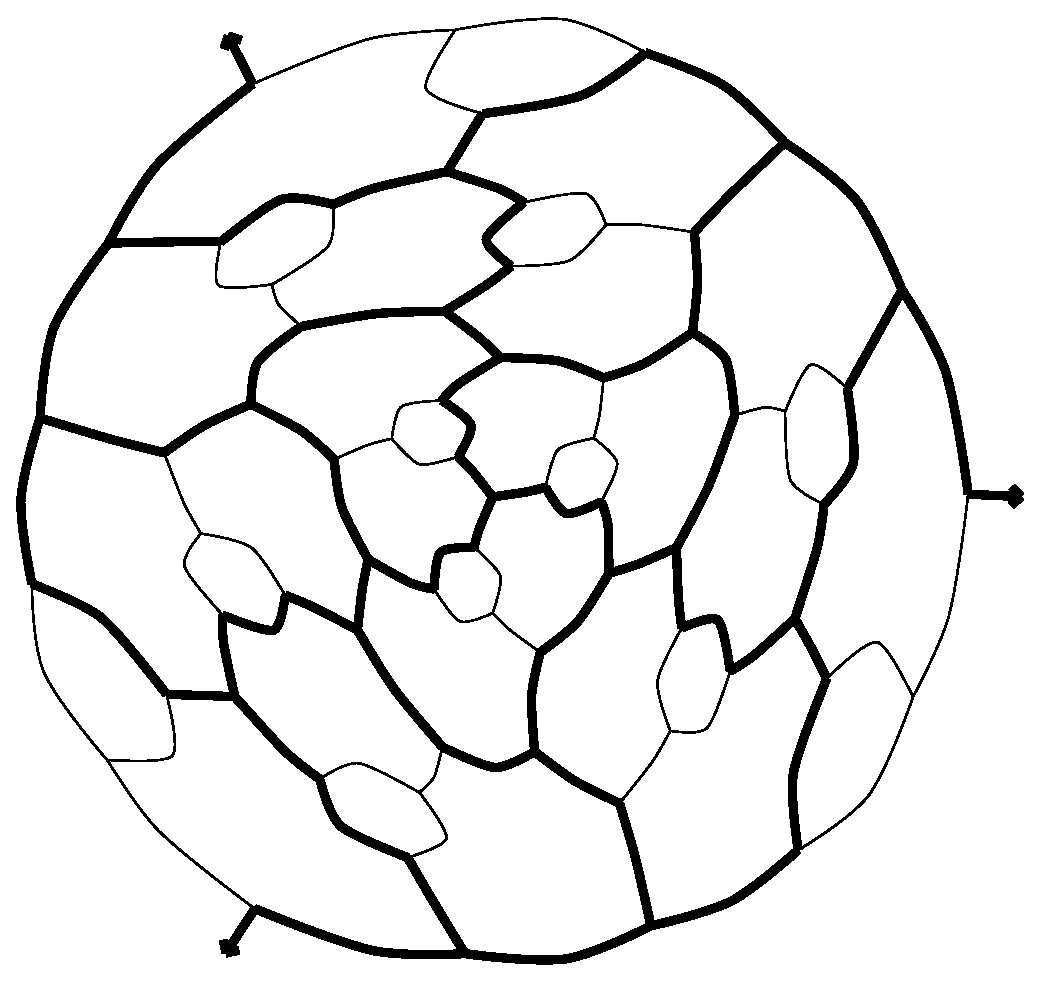
\epsfig{height=24mm, file=EPSdatabase/CASE_g0_k3_n68_-_3_12_-_7_24/PLOT_1_PL_69_T_1_-_3_T.eps}\par
$68$, $T$
\end{minipage}
\begin{minipage}[b]{2.7cm}\centering
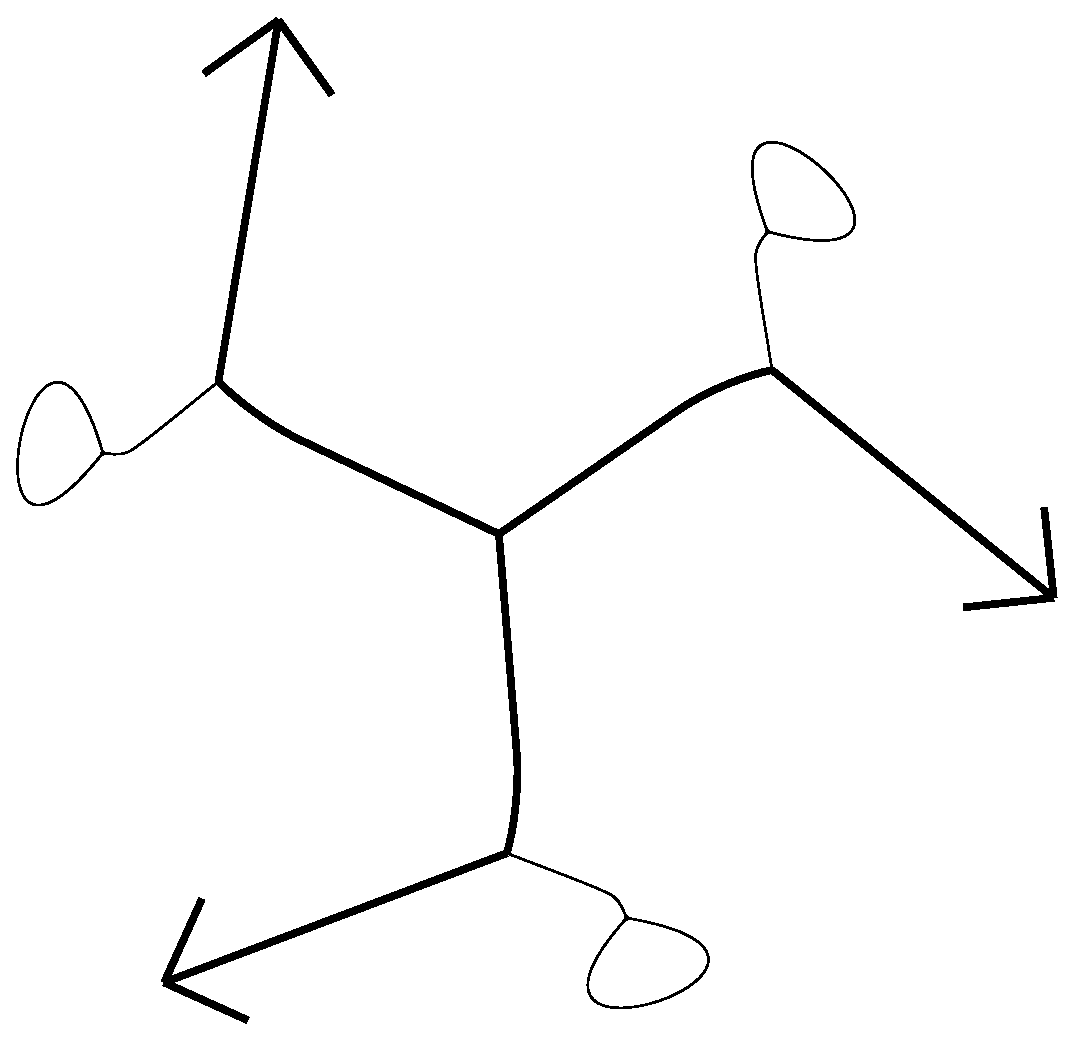
\epsfig{height=2.4cm, file=EPSexceptional/CASE_g0_k3_n8_-_1_3_-_7_3/PLOT_1_PL_1_C3_1_-_1_C3.eps}\par
8, $C_3$
\end{minipage}
\begin{minipage}[b]{2.6cm}\centering
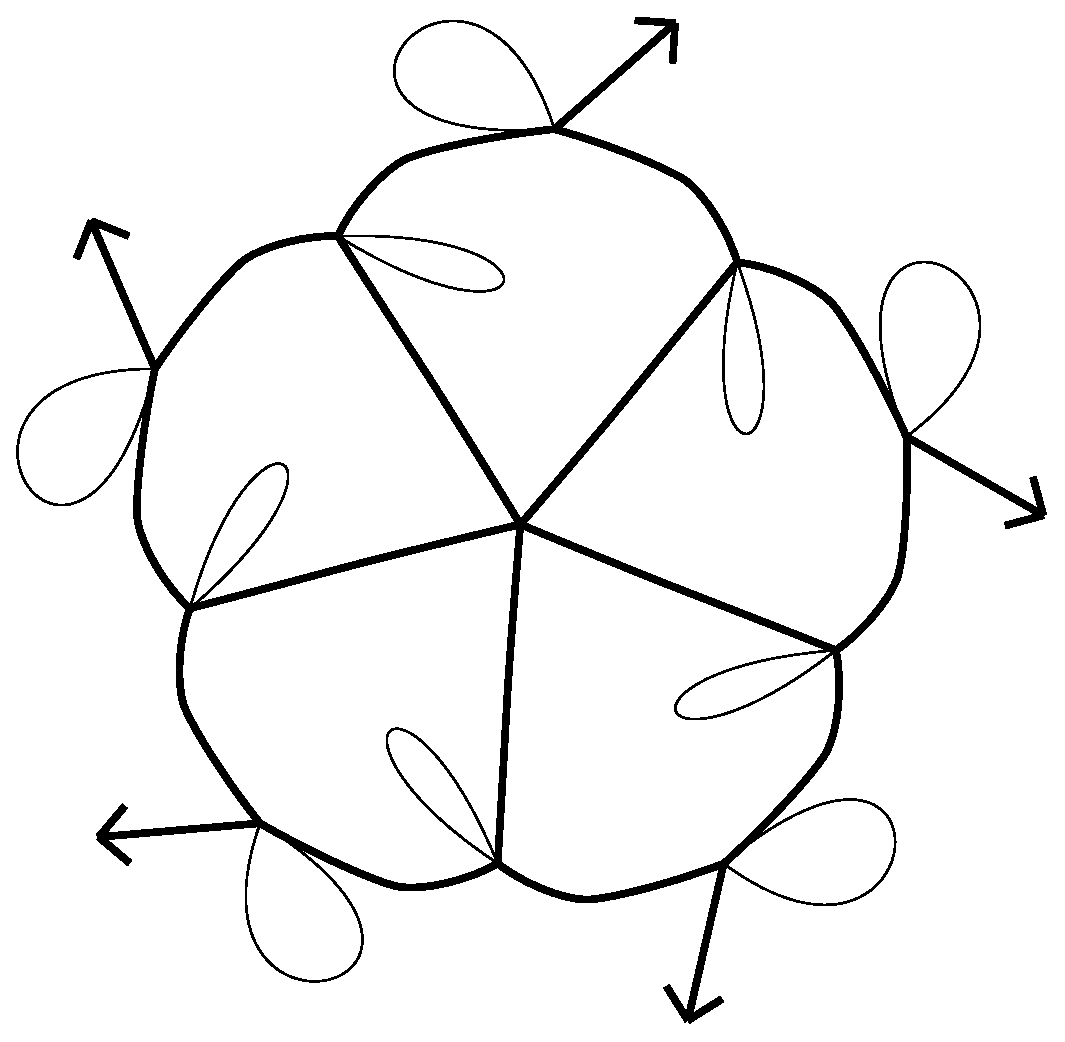
\epsfig{height=2.4cm, file=EPSexceptional/CASE_g0_k5_n12_-_1_10_-_5_10/PLOT_1_PL_3_D5_1_-_1_D5.eps}\par
12, $D_5$
\end{minipage}
\begin{minipage}[b]{2.5cm}\centering
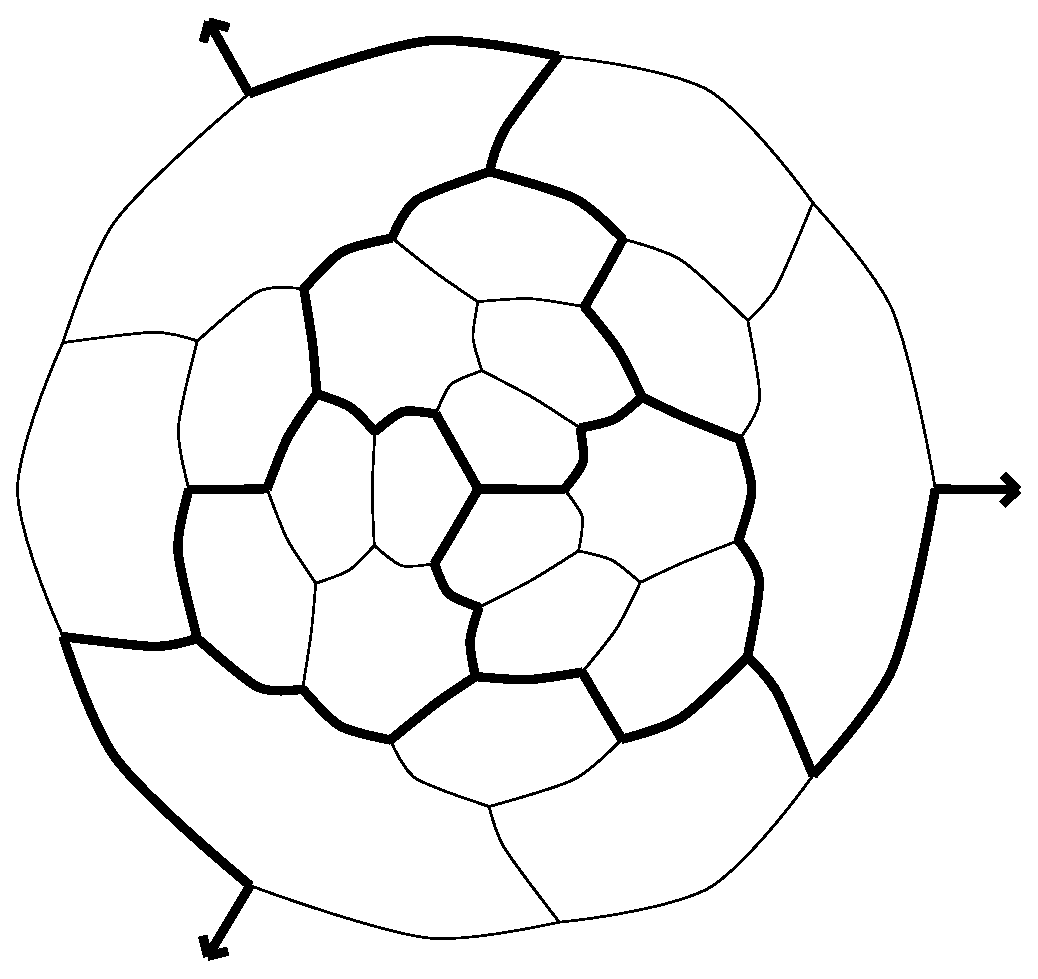
\epsfig{height=24mm, file=EPSdatabase/CASE_g0_k3_n44_-_5_18_-_7_6/PLOT_2_PL_11_D3h_2_-_1_D3.eps}\par
44 $D_{3h}$($D_3$)
\end{minipage}

\end{center}



\end{frame}




\begin{frame}
  \frametitle{When do lego exists?}

Plane graph case:
\begin{itemize}
\item In the elliptic cases we have a finite number of graphs to consider. Easy.
\item In the parabolic cases:
  \begin{itemize}
  \item If $\frac{p_a}{p_b}$ is integer then again a finite list of graphs to consider.
  \item If $\frac{p_b}{p_a}$ is integer then we have an infinite set of possibilities and existence can be proved in all of them.
  \end{itemize}
\item In the hyperbolic cases:
  \begin{itemize}
  \item If $\frac{p_b}{p_a}$ is integer then we can prove that there are only a finite number of possibilities.
  \item If $\frac{p_a}{p_b}$ is integer then a priori infinite number of possibilities but existence is not proved.
  \end{itemize}
\end{itemize}
Torus case:
\begin{itemize}
\item If $\frac{p_b}{p_a}$ is integer then we can prove that there are only a finite number of possibilities.
\item If $\frac{p_a}{p_b}$ is integer then a priori infinite number of possibilities but existence is not proved.
\end{itemize}

\end{frame}
  







\begin{frame}
  \frametitle{Classification results I}

For a hyperbolic $(\{a,b\},k)$-sphere the number $\frac{p_b}{p_a}$ is an integer if and only if its $p$-vector is either $(p_1, p_3)=(\frac{k}{2}, \frac{k}{2})$, $k\geq 8$, $k\equiv 0\pmod 4$ or one of $42$ cases:
  
\begin{center}
\begin{minipage}[b]{5cm}
\begin{tabular}{||c|c|c|c||}
\hline\hline
  k & a,b  & v   &$(p_a,p_b)$\\
\hline\hline
  3 & 3,7  & 20  & (6,6)   \\
  3 & 3,7  & 68  & (12,24) \\
  3 & 3,8  & 44  & (12,12) \\
  3 & 4,7  & 44  & (12,12) \\
  3 & 2,7  & 12  & (4,4)   \\
  3 & 2,7  & 32  & (6,12)  \\
  3 & 2,7  & 92  & (12,36) \\
  3 & 2,8  & 20  & (6,6)   \\
  3 & 2,9  & 44  & (12,12) \\
  4 & 2,5  & 14  & (8,8)   \\
  5 & 2,4  & 12  & (10,10) \\
  7 & 2,3  & 16  & (14,28) \\
\hline\hline
\end{tabular}
\end{minipage}
\begin{minipage}[b]{5cm}
\begin{tabular}{||c|c|c|c||}
\hline\hline
  k & a,b  & v   &$(p_a,p_b)$\\
\hline\hline
  7 & 2,3  & 44  & (28,84) \\
  8 & 2,3  & 10  & (16,16) \\
  9 & 2,3  & 20  & (36,36) \\
  3 & 1,7  & 8   & (3,3)   \\
  3 & 1,7  & 20  & (4,8)   \\
  3 & 1,7  & 44  & (6,18)  \\
  3 & 1,7  & 116 & (12,48) \\
  3 & 1,8  & 12  & (4,4)   \\
  3 & 1,8  & 68  & (12,24) \\
  3 & 1,9  & 20  & (6,6)   \\
  3 & 1,10 & 44  & (12,12) \\
  4 & 1,5  & 6   & (4,4)   \\
\hline\hline
\end{tabular}
\end{minipage}
\end{center}

\end{frame}

\begin{frame}
  \frametitle{Classification results II}

\begin{center}
\begin{minipage}[b]{5cm}
\begin{tabular}{||c|c|c|c||}
\hline\hline
  k & a,b  & v   &$(p_a,p_b)$\\
\hline\hline
  4 & 1,5  & 22  & (8,16)  \\
  4 & 1,6  & 14  & (8,8)   \\
  5 & 1,4  & 4   & (4,4)   \\
  5 & 1,4  & 52  & (20,60) \\
  5 & 1,5  & 12  & (10,10) \\
  6 & 1,4  & 5   & (6,6)   \\
  7 & 1,3  & 4   & (4,8)   \\
  7 & 1,3  & 16  & (7,35)  \\
  7 & 1,3  & 44  & (14,98) \\
\hline\hline
\end{tabular}
\end{minipage}
\begin{minipage}[b]{5cm}
\begin{tabular}{||c|c|c|c||}
\hline\hline
  k & a,b  & v   &$(p_a,p_b)$\\
\hline\hline
  7 & 1,3  & 100 & (28,224)\\
  8 & 1,3  & 10  & (8,24)  \\
  8 & 1,3  & 26  & (16,64) \\
  8 & 1,4  & 10  & (16,16) \\
  9 & 1,3  & 20  & (18,54) \\
  9 & 1,4  & 20  & (36,36) \\
 10 & 1,3  & 7   & (10,20) \\
 12 & 1,3  & 14  & (24,48) \\
 13 & 1,3  & 28  & (52,104)\\
\hline\hline
\end{tabular}
\end{minipage}

\end{center}
Notes:
\begin{itemize}
\item Of those cases, only the $(\{1,3\},7)$-spheres with $16$ vertices cannot be realized as a lego.
\end{itemize}

\end{frame}





\begin{frame}
  \frametitle{Classification results III}

The  parameters of putative $(\{a,b\};k)$-tori with integer $\frac{p_b}{p_a}$
\begin{center}
{\small
\begin{tabular}{||c|c|c|c||c|c|c|c||c|c|c|c||}
\hline\hline
 k  & a,b & v & $\frac{p_b}{p_a}$  & k  & a,b & v & $\frac{p_b}{p_a}$  & k  & a,b & v & $\frac{p_b}{p_a}$ \\
\hline
\hline
 3  & 3,7  & 8$p_3$  & 3 & 4  & 2,5  & $3p_2$           & 2 & 4  & 1,5  & $4p_1$  & 3\\
 3  & 3,9  & 4$p_3$  & 1 & 4  & 2,6  & $2p_2$           & 1 & 4  & 1,7  & $2p_1$  & 1\\
 3  & 4,7  & 6$p_4$  & 2 & 5  & 2,4  & $2p_2$           & 2 & 6  & 1,4  & $\frac{3}{2}p_1$ & 2\\
 3  & 4,8  & 4$p_4$  & 1 & 6  & 2,4  & $p_2$            & 1 & 6  & 1,5  & $p_1$   & 1\\
 3  & 5,7  & 4$p_5$  & 1 & 7  & 2,3  & $2p_2$           & 4 & 7  & 1,3  & $4p_1$  & 9\\
 4  & 3,5  & 2$p_3$  & 1 & 8  & 2,3  & $p_2$            & 2 & 8  & 1,3  & $2p_1$  & 5\\
 3  & 2,7  & 10$p_2$ & 4 & 10 & 2,3  & $\frac{1}{2}p_2$ & 1 & 10 & 1,3  & $p_1$   & 3\\
 3  & 2,8  & $6p_2$  & 2 & 3  & 1,7  & $12p_1$          & 5 & 10 & 1,4  & $\frac{1}{2}p_1$ & 1\\
 3  & 2,10 & $4p_2$  & 1 & 3  & 1,11 & $4p_1$           & 1 & 14 & 1,3  &$\frac{1}{2}p_1$ &2\\
\hline\hline
\end{tabular}
}
\end{center}
  

\end{frame}


  



%\begin{frame}\frametitle{Parabolic lego-like   $(\{a,b\}; k)$-$\mathbb{S}^2$: computations}
%\vspace{-4mm}
%\begin{center}
%\tiny
%For  $(3,6;3),(2,6;3),(2,4;4)$, all computed spheres are lego-like.
%\begin{tabular}{||c|c|c|c|c|c|c|c|c||}
%\hline \hline
%k & lego & $(p_a, p_b)$ & v & nbG/real. & nbCases/real. & nbCasesRed/real. & Max./Min. & total\\
%\hline
%3 & $4^{3}6$ & (6,2) & 12 & $1/1$ & $9/3$ & $7/3$ & $3/3$ & 3\\
%3 & $4^{2}6$ & (6,3) & 14 & $1/1$ & $4/2$ & $4/2$ & $2/2$ & 2\\
%3 & $46$ & (6,6) & 20 & $3/3$ & $1/1$ & $1/1$ & $9/2$ & 13\\
%3 & $46^{2}$ & (6,12) & 32 & $8/8$ & $5/5$ & $4/4$ & $18/3$ & 59\\
%\textcolor{red}{3} & $\textcolor{red}{46^{3}}$ &\textcolor{red}{(6,18)} &\textcolor{red}{ 44} & $ \textcolor{red}{ 14/14}$ & $21/20$ & $13/13$ & $36/2$ & 132\\
%3 & $46^{4}$ & (6,24) & 56 & $23/20$ & $103/86$ & $57/53$ & $60/1$ & 324\\
%\hline
%3 & $5^{6}6$ & (12,2) & 24 & $1/1$ & $628/31$ & $328/31$ & $31/31$ & 31\\
%3 & $5^{4}6$ & (12,3) & 26 & $1/1$ & $62/6$ & $36/6$ & $6/6$ & 6\\
%3 & $5^{3}6$ & (12,4) & 28 & $2/2$ & $18/16$ & $11/11$ & $25/13$ & 38\\
%3 & $5^{2}6$ & (12,6) & 32 & $6/6$ & $5/5$ & $4/4$ & $13/4$ & 45\\
%\textcolor{red}{3} & $\textcolor{red}{56}$ &\textcolor{red}{(12,12)} & \textcolor{red}{44} & $\textcolor{red}{89/89}$ & $1/1$ & $1/1$ & $627/1$ & 11846\\
%3 & $56^{2}$ & (12,24) & 68 & $6332/4281$ & $5/5$ & $4/4$ & $128/1$ & 36760\\
%3 & $56^{3}$ & (12,36) & 92 & $126409/5520$ & $25/25$ & $15/15$ & $287/1$ & 18691\\
%\hline
%4 & $3^{4}4$ & (8,2) & 8 & $1/1$ & $20/5$ & $13/5$ & $5/5$ & 5\\
%4 & $3^{2}4$ & (8,4) & 10 & $2/2$ & $4/4$ & $3/3$ & $8/4$ & 12\\
%\textcolor{red}{4} & $\textcolor{red}{34}$ & \textcolor{red}{(8,8)} & \textcolor{red}{14} & $\textcolor{red}{8/8}$ & $1/1$ & $1/1$ & $11/1$ & 27\\
%4 & $34^{2}$ & (8,16) & 22 & $51/43$ & $4/4$ & $3/3$ & $14/1$ & 268\\
%4 & $34^{3}$ & (8,24) & 30 & $218/69$ & $16/16$ & $10/10$ & $20/1$ & 311\\
%4 & $34^{4}$ & (8,32) & 38 & $650/118$ & $59/54$ & $33/32$ & $30/1$ & 412\\
%4 & $34^{5}$ & (8,40) & 46 & $1653/327$ & $229/157$ & $121/94$ & $77/1$ & 1312\\
%\hline
%6 & $2^{3}3$ & (6,2) & 3 & $1/1$ & $4/2$ & $3/2$ & $2/2$ & 2\\
%\textcolor{red}{6} & $\textcolor{red}{23}$ &\textcolor{red}{(6,6)} &\textcolor{red}{ 5} & $\textcolor{red}{2/2}$ & $1/1$ & $1/1$ & $2/1$ & 3\\
%6 & $23^{2}$ & (6,12) & 8 & $12/10$ & $3/3$ & $2/2$ & $4/1$ & 22\\
%6 & $23^{3}$ & (6,18) & 11 & $16/9$ & $7/6$ & $4/4$ & $5/1$ & 19\\
%6 & $23^{4}$ & (6,24) & 14 & $42/18$ & $22/18$ & $12/10$ & $10/1$ & 52\\
%6 & $23^{5}$ & (6,30) & 17 & $48/11$ & $61/27$ & $32/17$ & $28/1$ & 55\\
%6 & $23^{6}$ & (6,36) & 20 & $100/26$ & $180/89$ & $93/57$ & $29/1$ & 179\\
%\hline \hline
%\end{tabular}
%\end{center}
%\end{frame}









%\begin{frame}
%  \frametitle{Some $(\{2,3\}, 6)$-spheres lego}
%\begin{center}\begin{minipage}[b]{19mm}\centering
%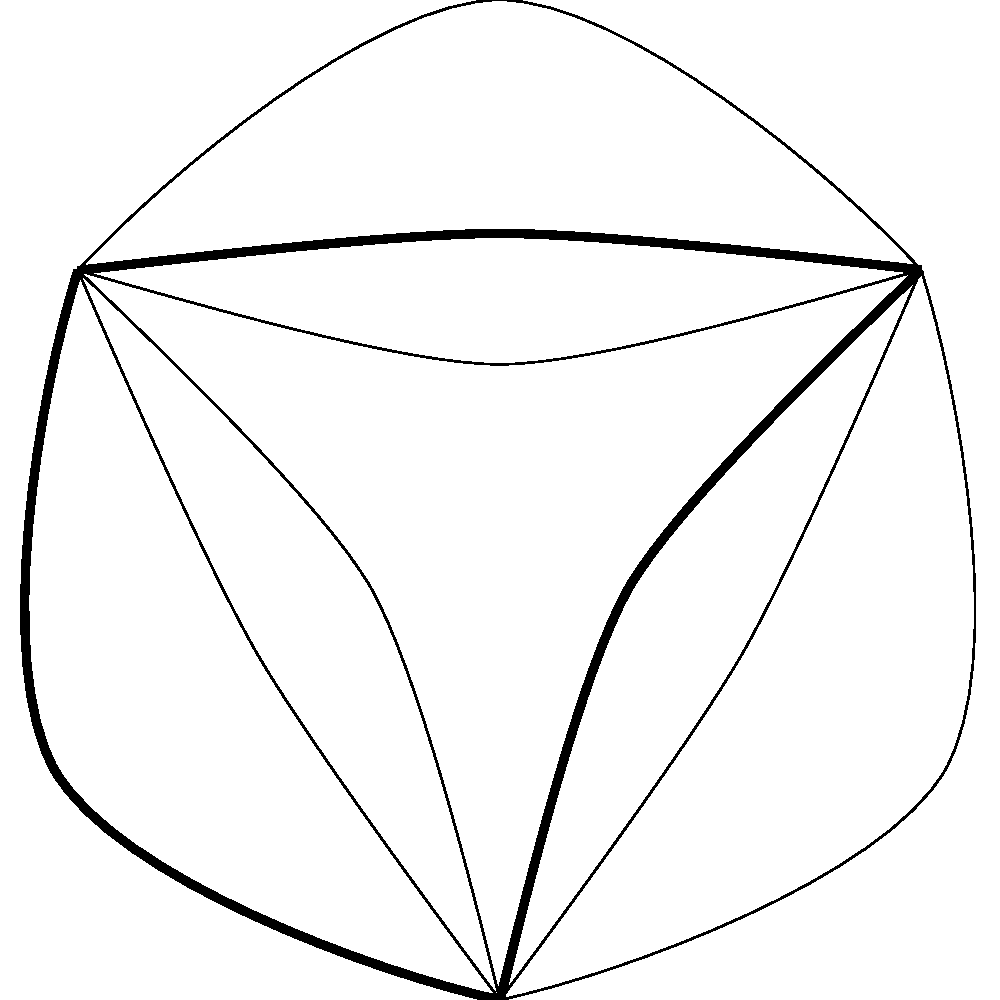
\epsfig{height=19mm, file=PDFdatabase/CASE_g0_k6_n3_-_2_6_-_3_2/PLOT_1_PL_1_D3h_2_-_1_C2.pdf}
%\par    $3$, $D_{3h}$($C_{2}$) \end{minipage}
%\begin{minipage}[b]{20mm}\centering
%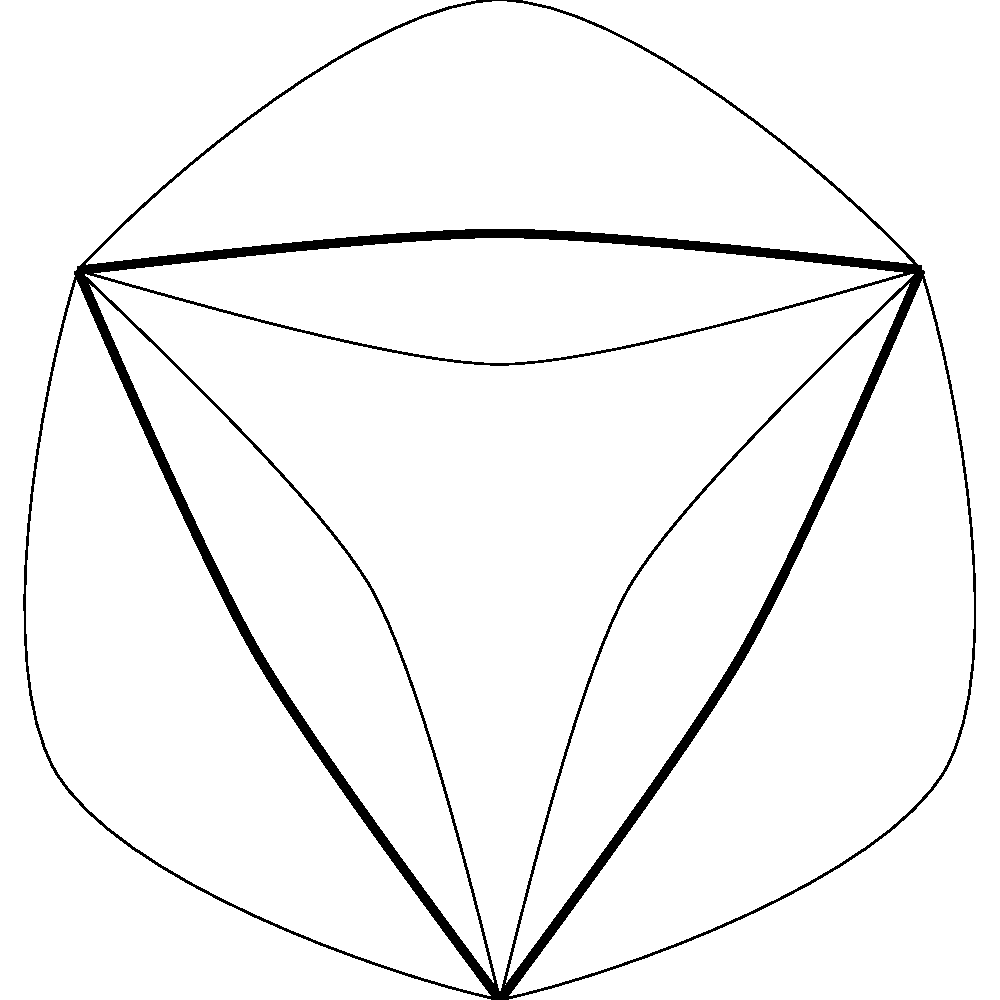
\epsfig{height=18mm, file=PDFdatabase/CASE_g0_k6_n3_-_2_6_-_3_2/PLOT_2_PL_1_D3h_3_-_1_D3h.pdf}
%\par$3$, $D_{3h}$($D_{3h}$) \end{minipage}
%\begin{minipage}[b]{19mm}\centering
%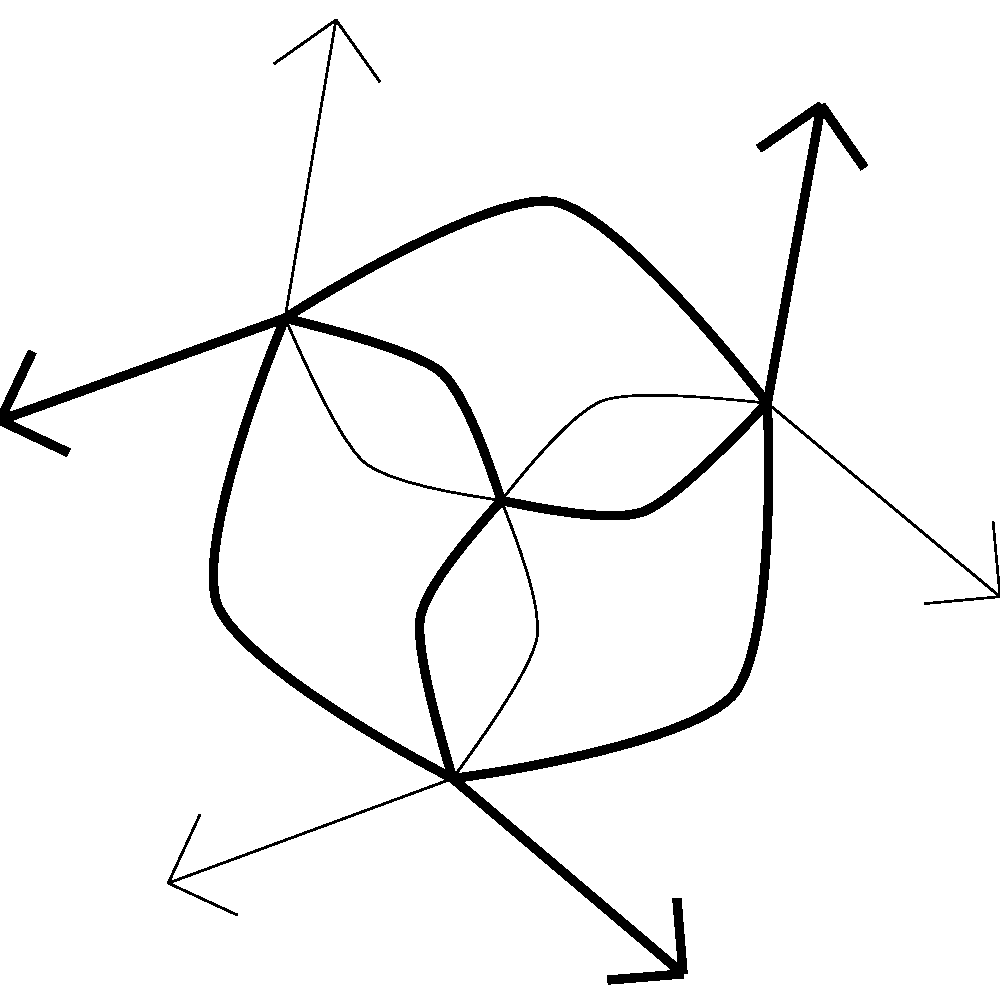
\epsfig{height=17mm, file=PDFdatabase/CASE_g0_k6_n5_-_2_6_-_3_6/PLOT_1_PL_2_D3h_1_-_1_D3.pdf}
%\par   $5$, $D_{3h}$($D_{3}$) \end{minipage}
%\begin{minipage}[b]{20mm}\centering
%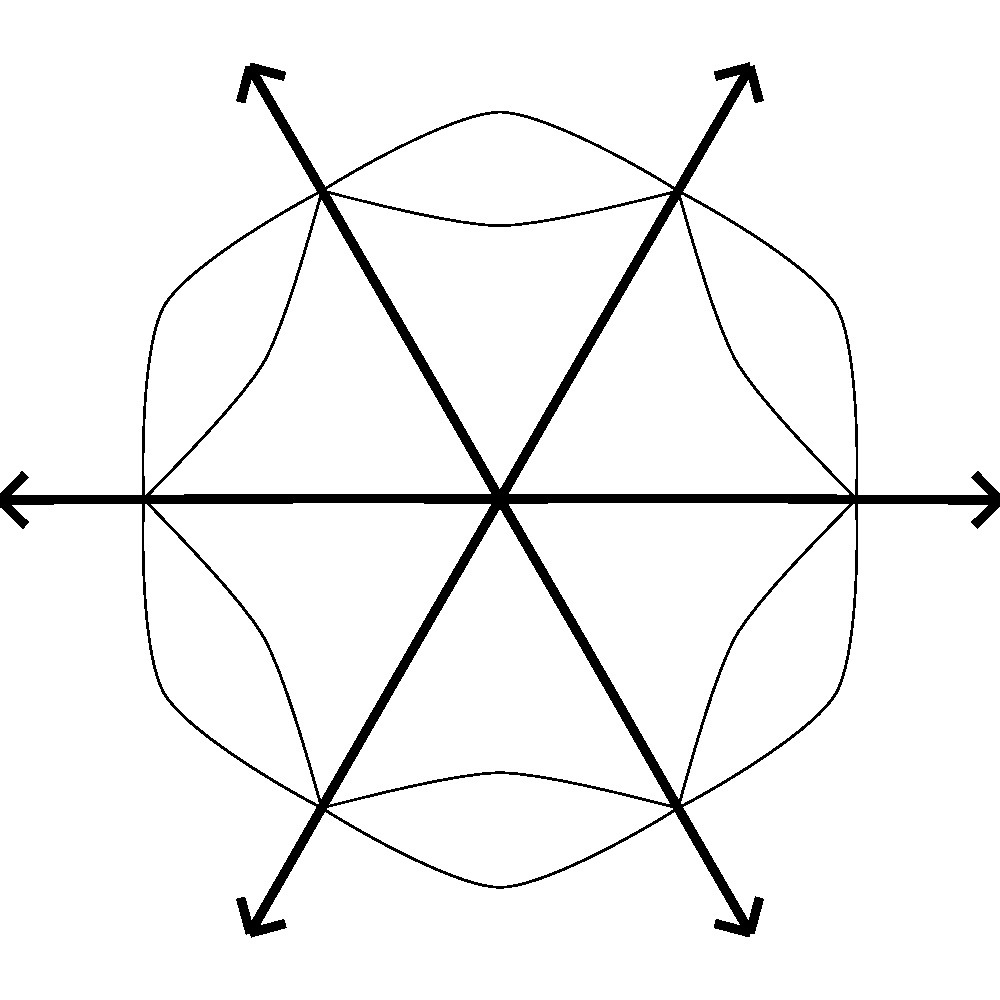
\epsfig{height=18mm, file=PDFdatabase/CASE_g0_k6_n8_-_2_6_-_3_12/PLOT_1_PL_10_D6h_1_-_1_D6h.pdf}
%\par   $8$, $D_{6h}$($D_{6h}$) \end{minipage}
%\begin{minipage}[b]{19mm}\centering
%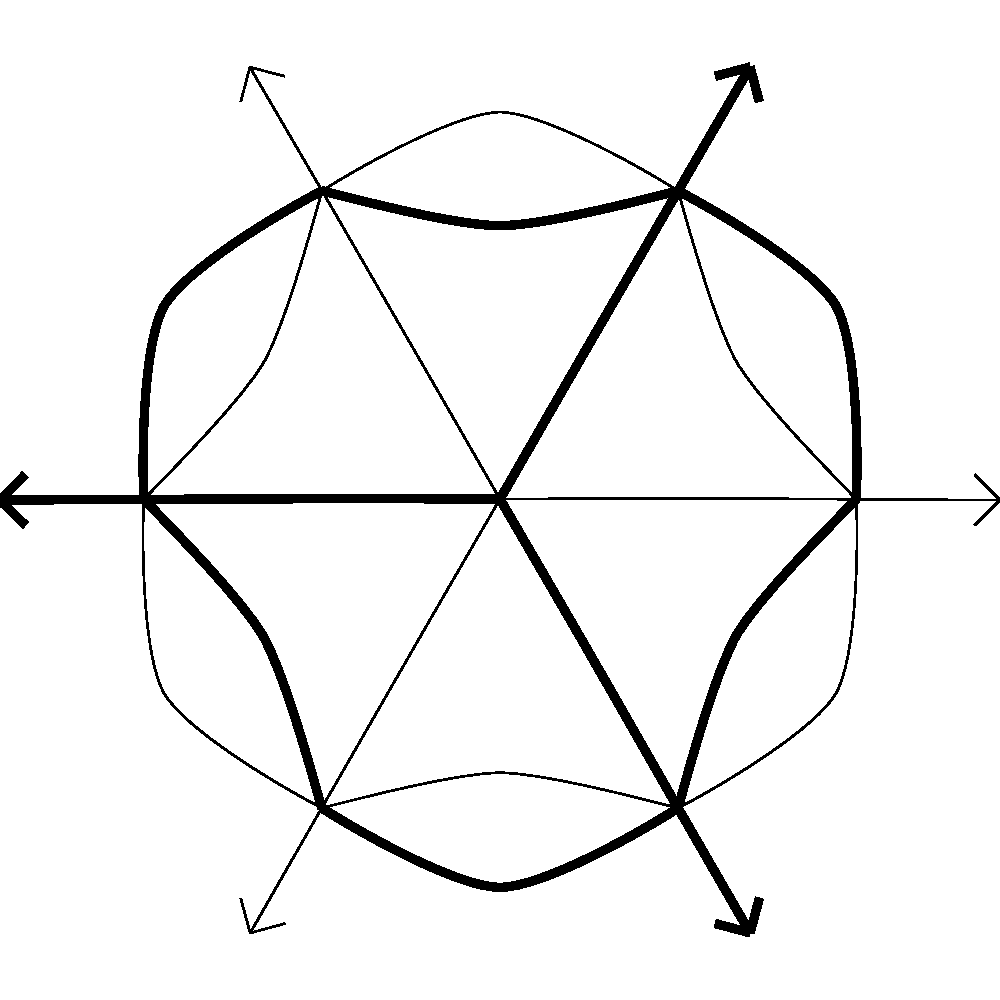
\epsfig{height=19mm, file=PDFdatabase/CASE_g0_k6_n8_-_2_6_-_3_12/PLOT_2_PL_10_D6h_2_-_1_D3.pdf}
%\par$8$, $D_{6h}$($D_{3}$) \end{minipage}
%\begin{minipage}[b]{19mm}\centering
%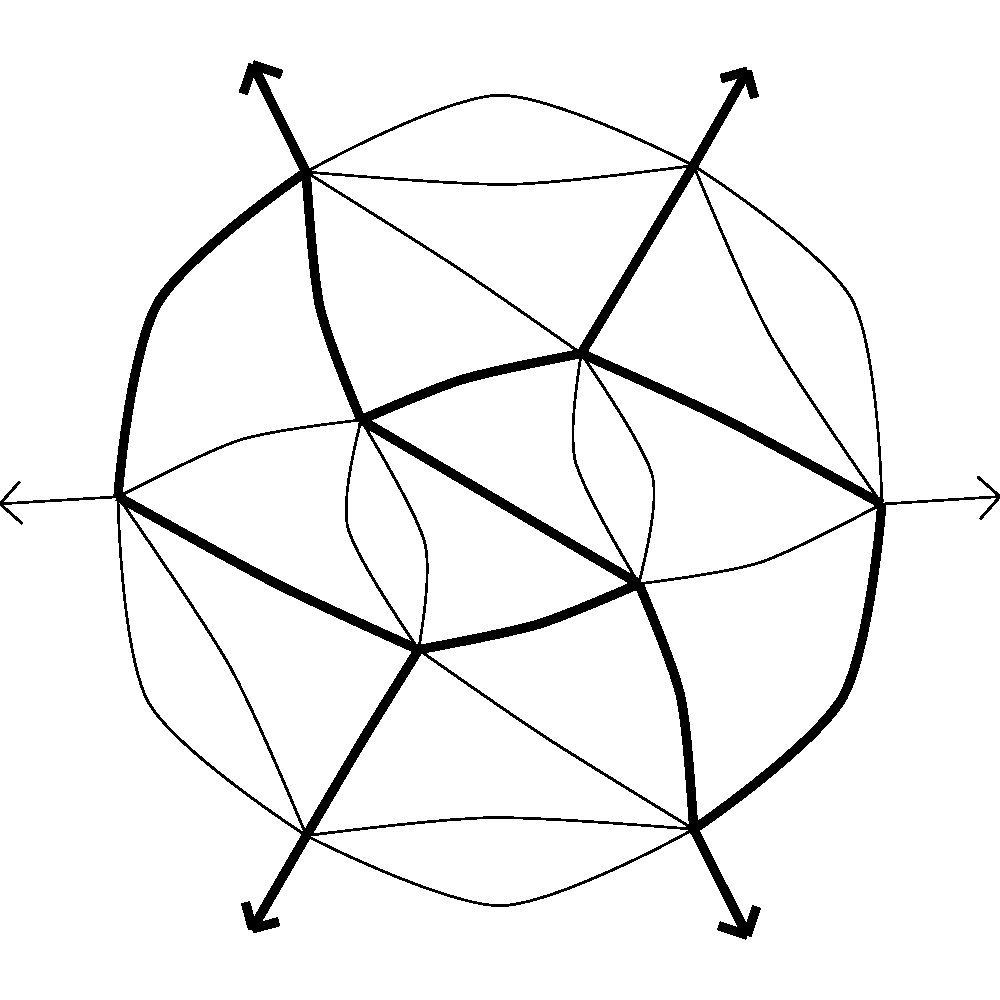
\epsfig{height=19mm, file=PDFdatabase/CASE_g0_k6_n11_-_2_6_-_3_18/PLOT_1_PL_5_C2_1_-_1_C2.pdf}
%\par   $11$, $C_{2}$($C_{2}$) \end{minipage}
%\begin{minipage}[b]{22mm}\centering
%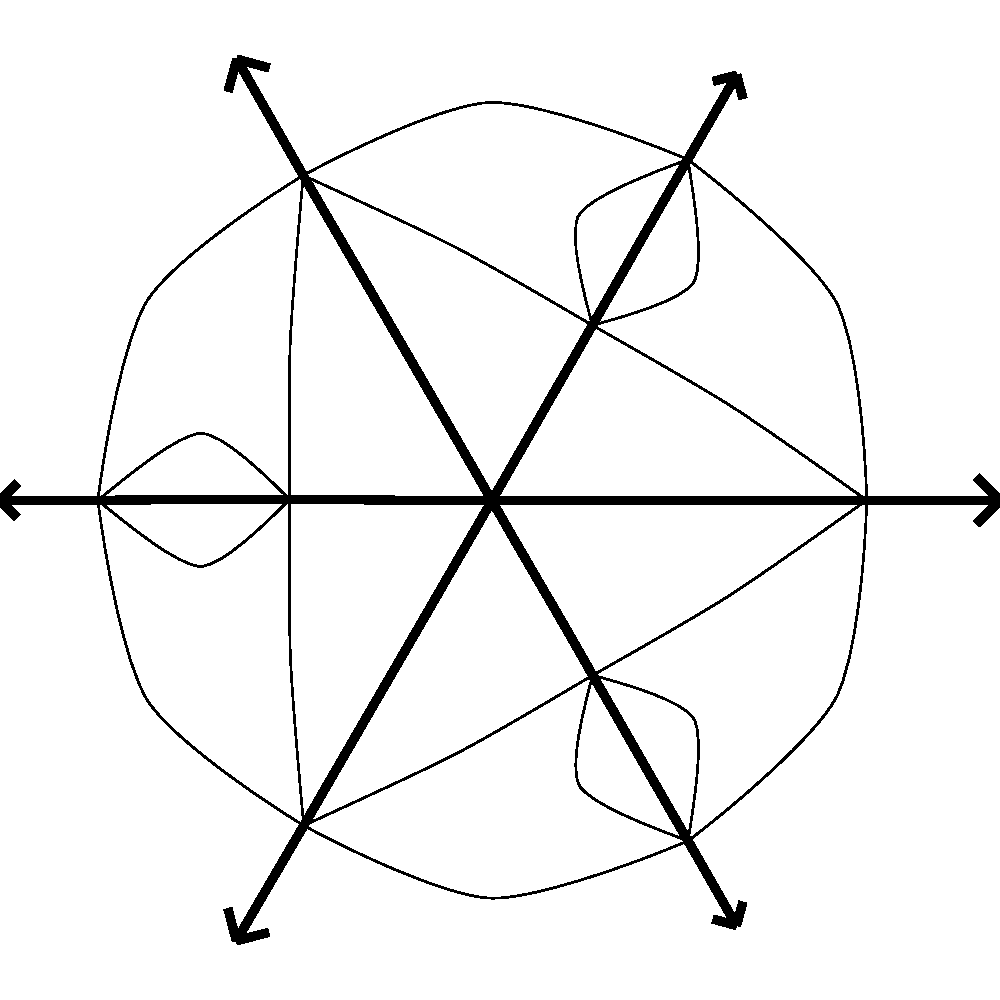
\epsfig{height=18mm, file=PDFdatabase/CASE_g0_k6_n11_-_2_6_-_3_18/PLOT_2_PL_11_D3h_2_-_1_D3h.pdf}
%\par$11$, $D_{3h}$($D_{3h}$) \end{minipage}
%\begin{minipage}[b]{20mm}\centering
%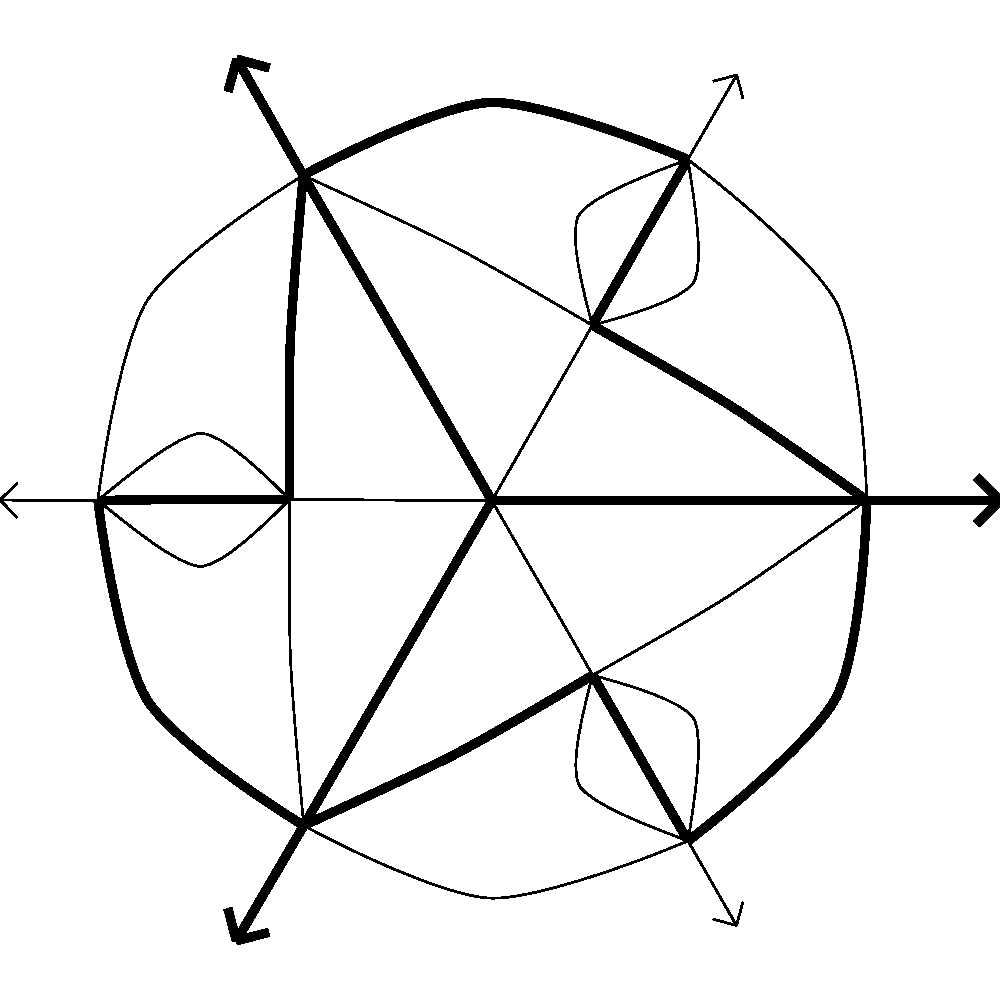
\epsfig{height=18mm, file=PDFdatabase/CASE_g0_k6_n11_-_2_6_-_3_18/PLOT_3_PL_11_D3h_3_-_1_D3.pdf}
%\par$11$, $D_{3h}$($D_{3}$) \end{minipage}
%\begin{minipage}[b]{20mm}\centering
%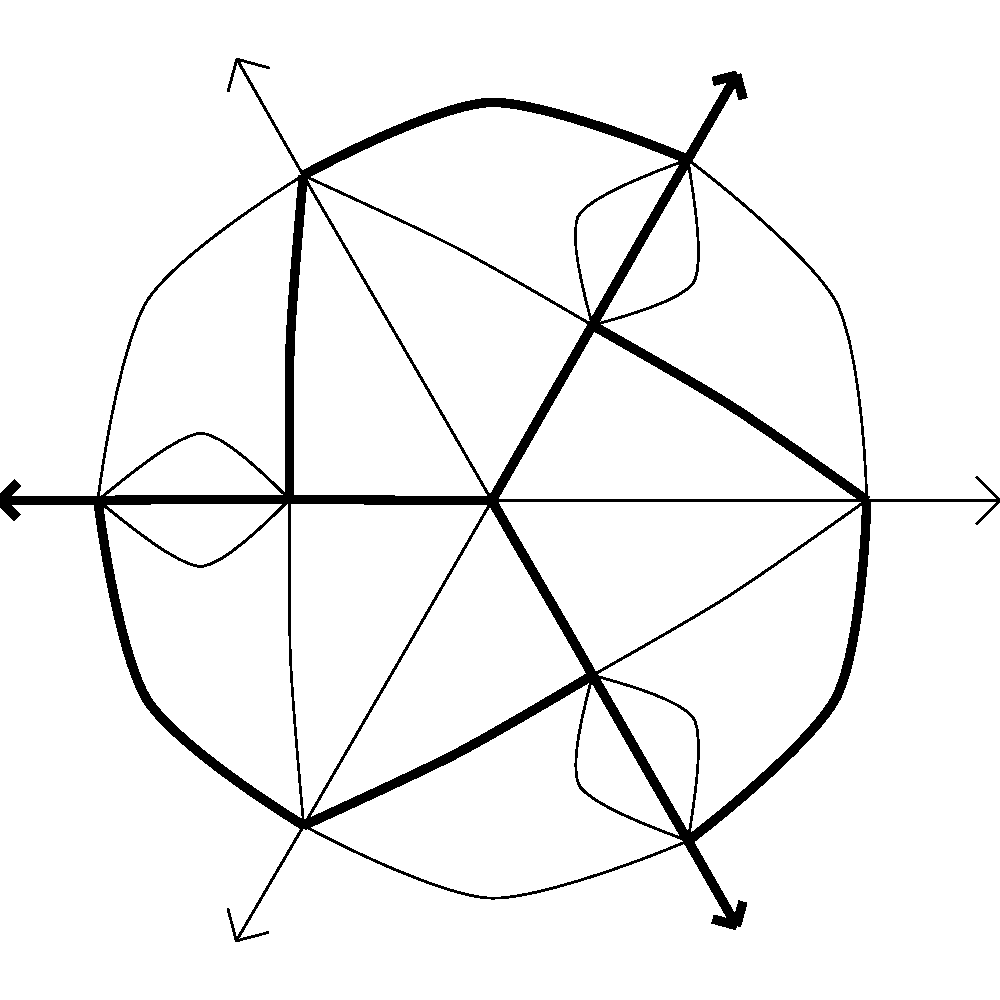
\epsfig{height=18mm, file=PDFdatabase/CASE_g0_k6_n11_-_2_6_-_3_18/PLOT_4_PL_11_D3h_4_-_1_D3.pdf}
%\par$11$, $D_{3h}$($D_{3}$) \end{minipage}
%\begin{minipage}[b]{19mm}\centering
%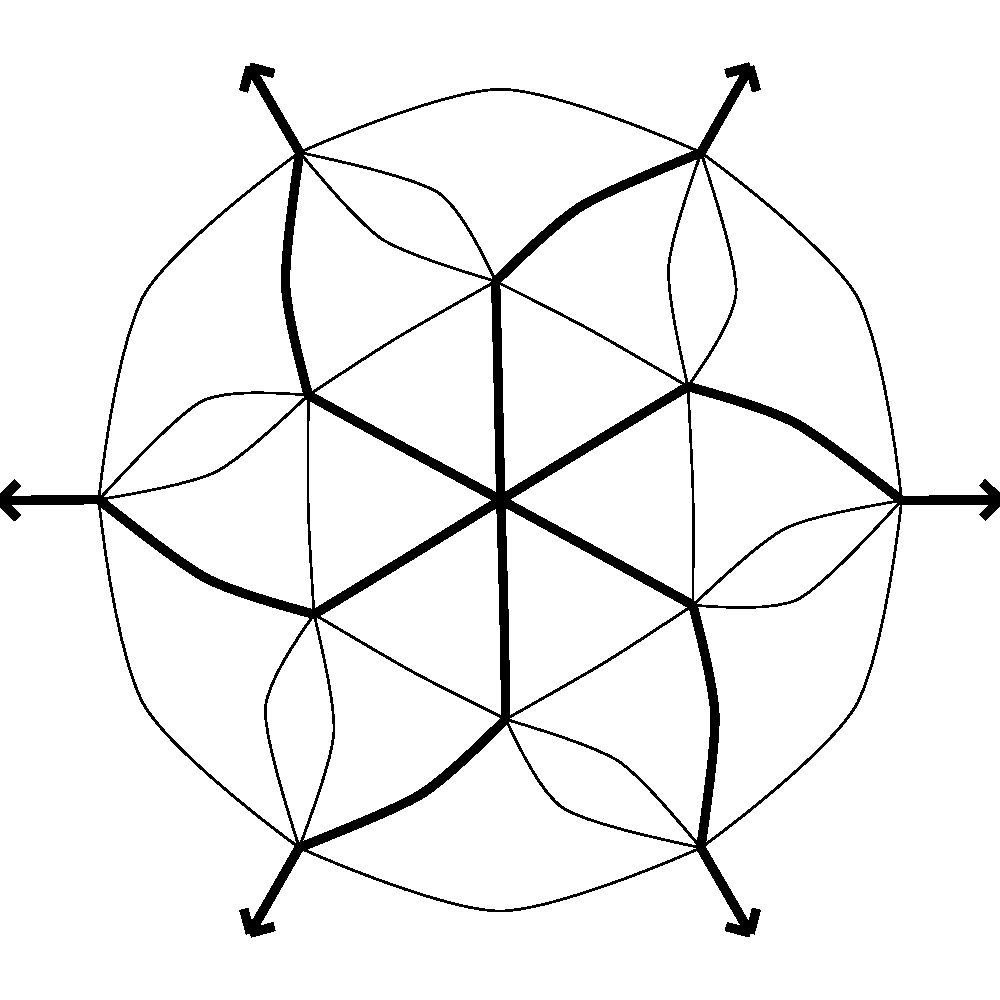
\epsfig{height=19mm, file=PDFdatabase/CASE_g0_k6_n14_-_2_6_-_3_24/PLOT_1_PL_42_D6_2_-_1_D6.pdf}
%\par   $14$, $D_{6}$($D_{6}$) \end{minipage}
%\begin{minipage}[b]{19mm}\centering
%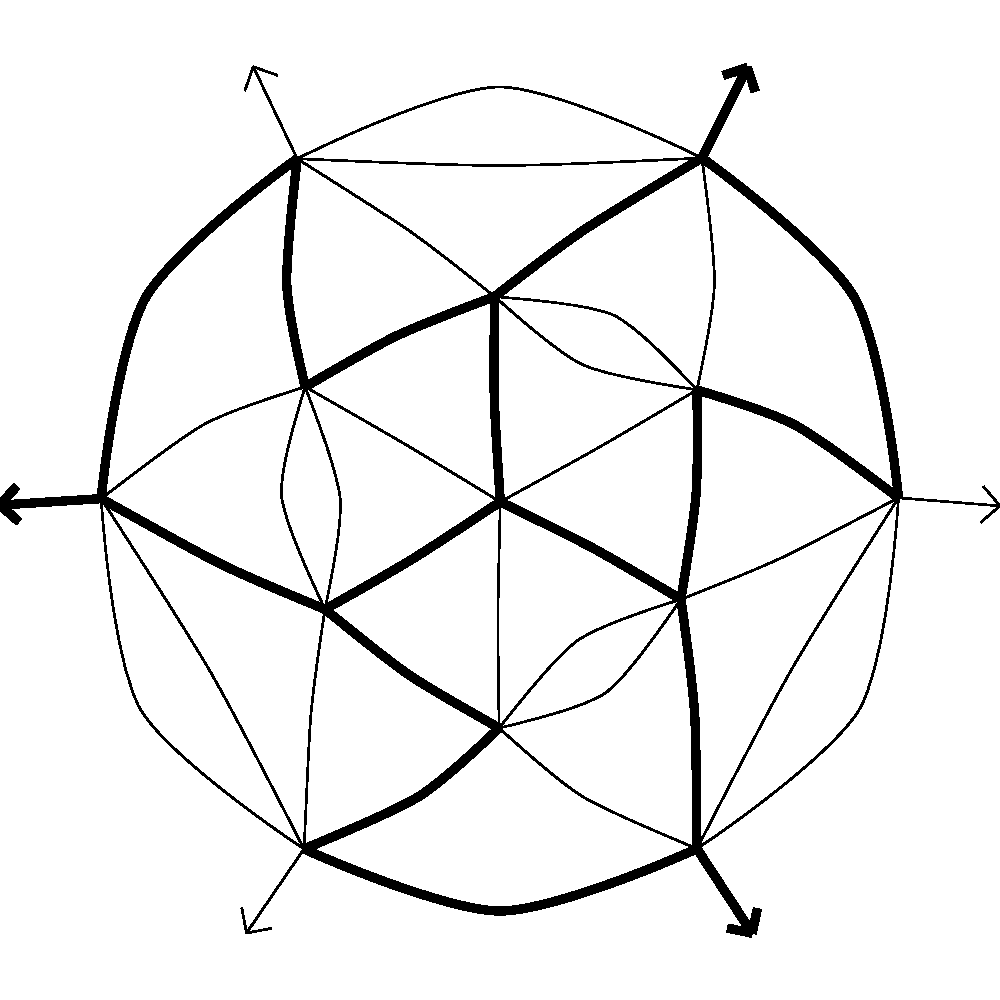
\epsfig{height=19mm, file=PDFdatabase/CASE_g0_k6_n14_-_2_6_-_3_24/PLOT_2_PL_34_D3_3_-_1_D3.pdf}
%\par$14$, $D_{3}$($D_{3}$) \end{minipage}
%\begin{minipage}[b]{19mm}\centering
%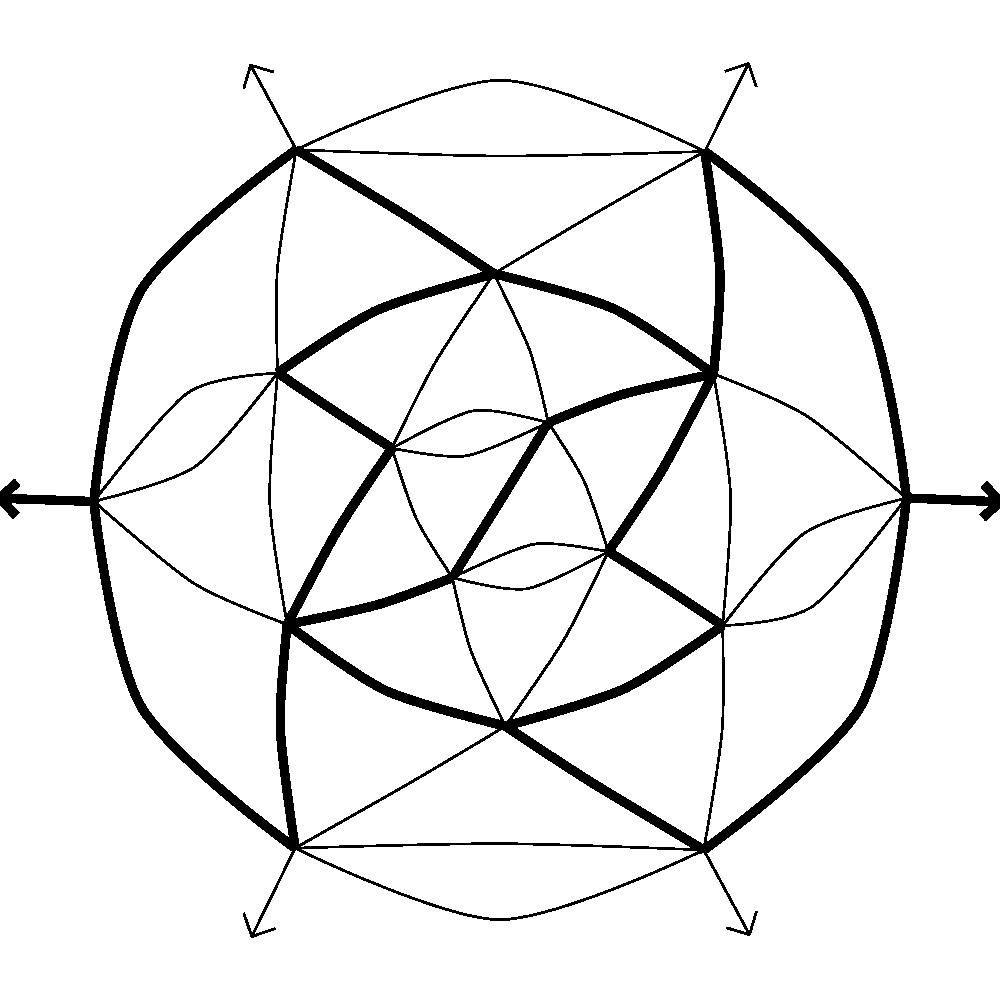
\epsfig{height=19mm, file=PDFdatabase/CASE_g0_k6_n17_-_2_6_-_3_30/PLOT_1_PL_23_C2_1_-_1_C2.pdf}
%\par  $17$, $C_{2}$($C_{2}$) \end{minipage}
%\begin{minipage}[b]{19mm}\centering
%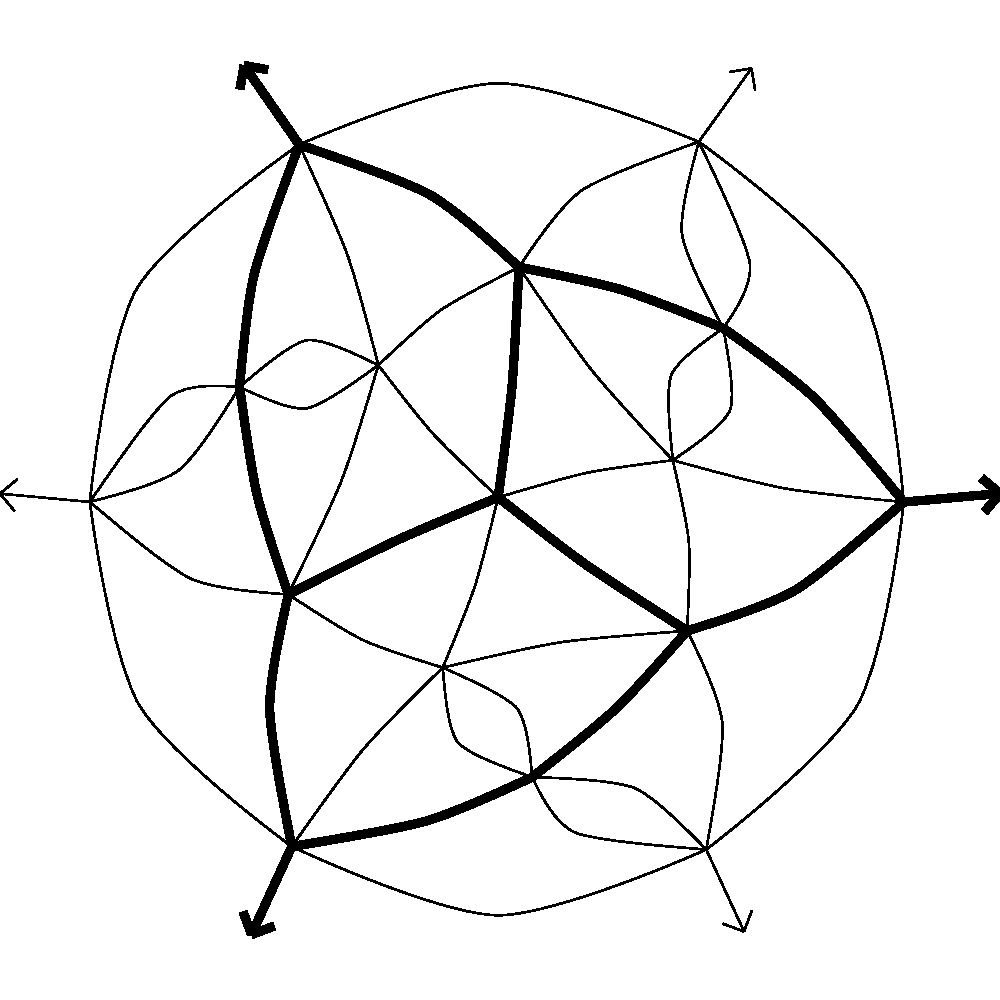
\epsfig{height=19mm, file=PDFdatabase/CASE_g0_k6_n17_-_2_6_-_3_30/PLOT_2_PL_9_D3_6_-_1_D3.pdf}
%\par$17$, $D_{3}$($D_{3}$) \end{minipage}
%\begin{minipage}[b]{20mm}\centering
%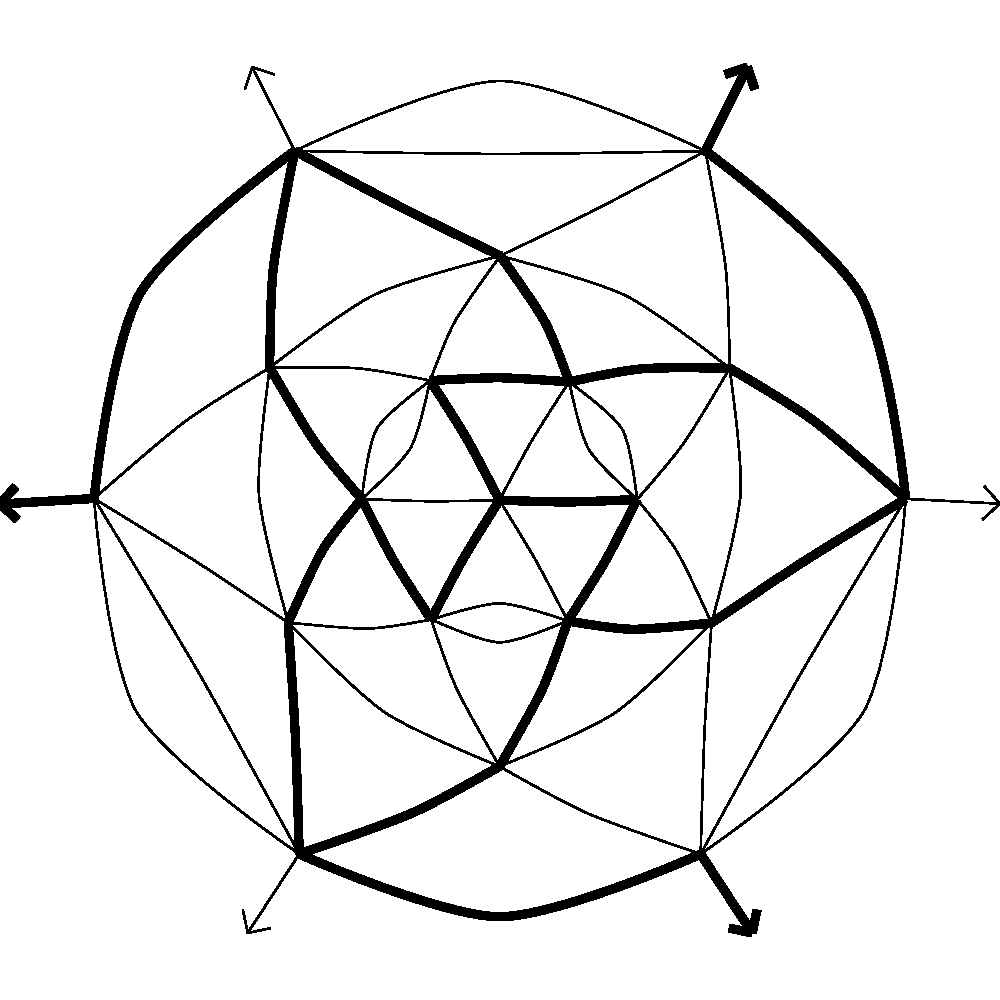
\epsfig{height=18mm, file=PDFdatabase/CASE_g0_k6_n20_-_2_6_-_3_36/PLOT_8_PL_32_D3d_14_-_1_S6.pdf}
%\par  $20$, $D_{3d}$($S_{6}$) \end{minipage}
%\begin{minipage}[b]{20mm}\centering
%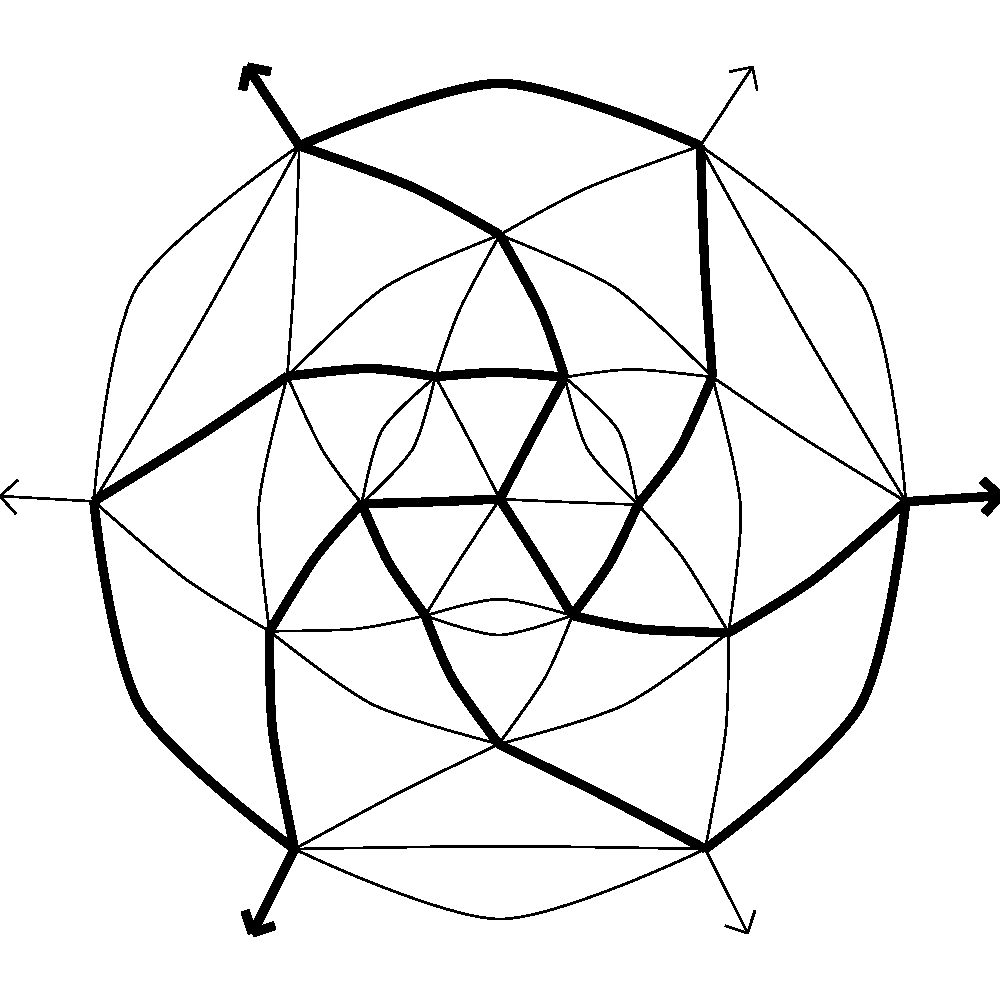
\epsfig{height=18mm, file=PDFdatabase/CASE_g0_k6_n20_-_2_6_-_3_36/PLOT_11_PL_88_D3h_19_-_1_D3.pdf}
%\par$20$, $D_{3h}$($D_{3}$) \end{minipage}
%\end{center}
%\end{frame}






%\begin{frame}
%  \frametitle{Some azulenoid $(\{5,7\};3)$-torus}
%\small
%\begin{center}
%\begin{minipage}[b]{2.4cm}\centering
%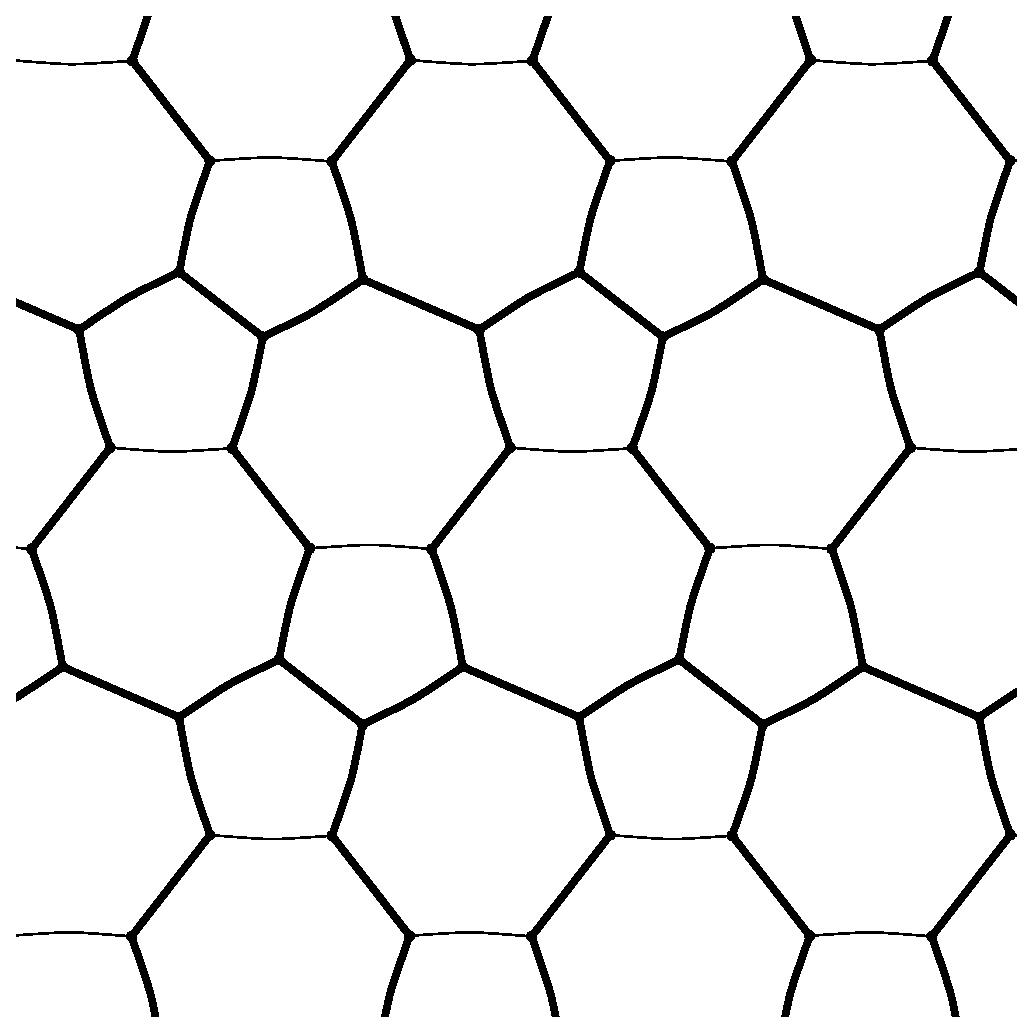
\epsfig{height=25mm, file=EPSdatabase/CASE_g1_k3_n8_-_5_2_-_7_2/PLOT_1_PL_1_c2mm_1_-_1_p2.eps}
%\par 
%8, $c2mm$ (p2)\\
%$\vec{p}$=$(2,2)$
%\end{minipage}
%\begin{minipage}[b]{2.8cm}\centering
%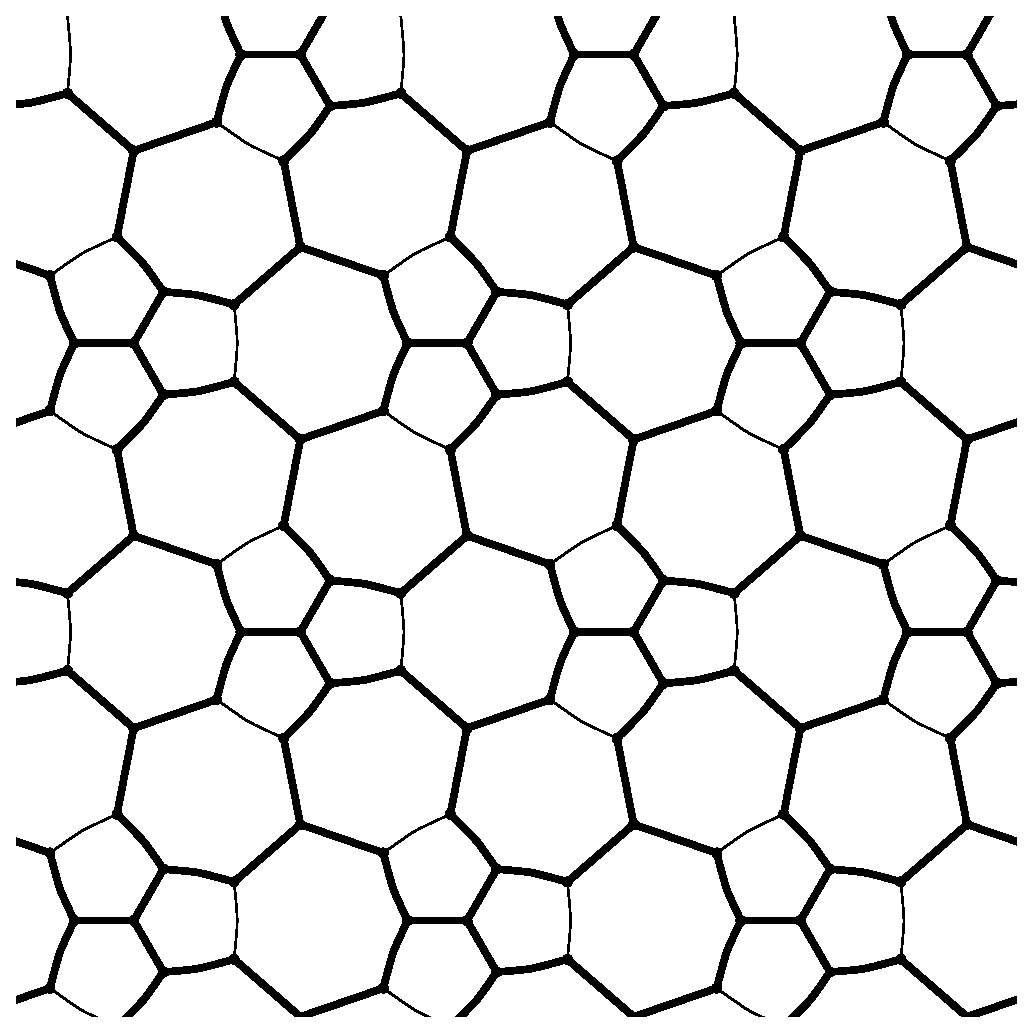
\epsfig{height=25mm, file=EPSdatabase/CASE_g1_k3_n12_-_5_3_-_7_3/PLOT_1_PL_1_p31m_1_-_3_p31m.eps}
%\par 
%12, $p31m$ (p31m)\\
%$\vec{p}$=$(3,3)$
%\end{minipage}
%\begin{minipage}[b]{2.8cm}\centering
%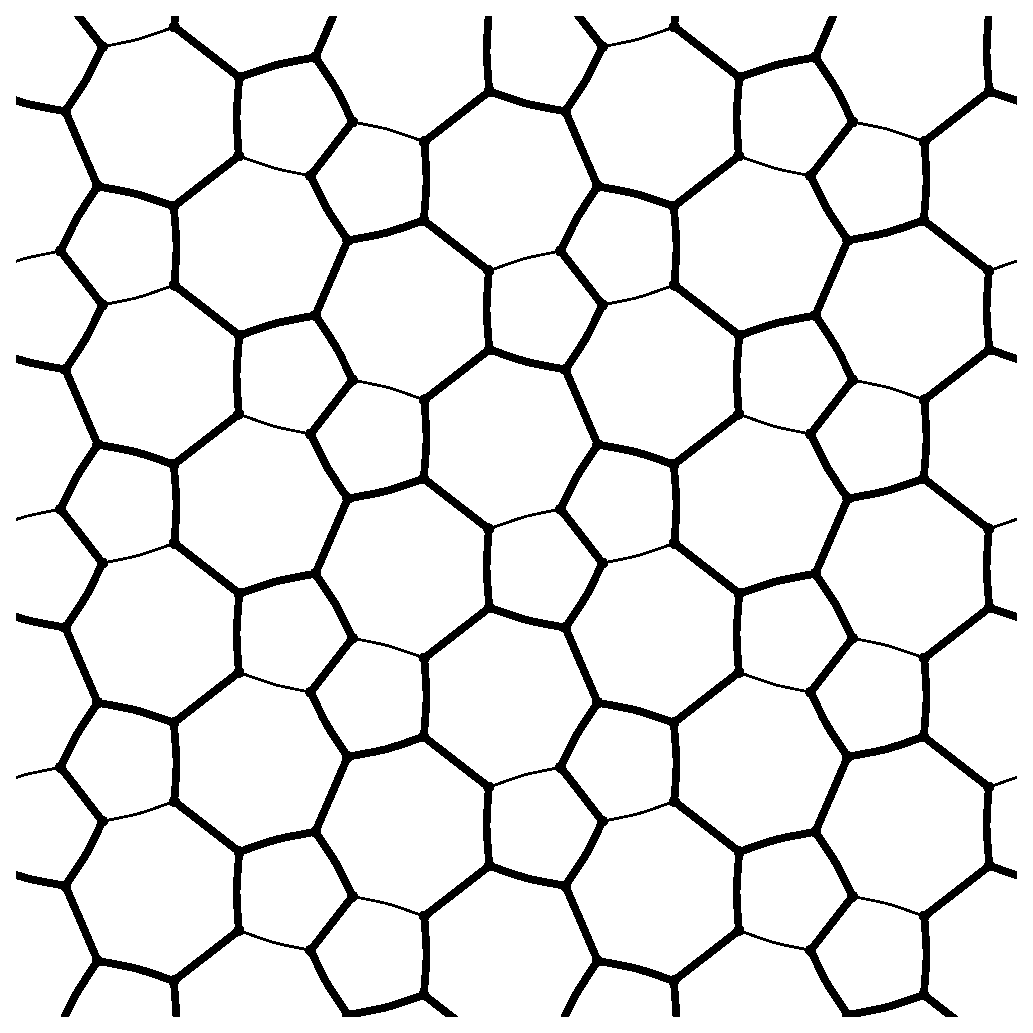
\epsfig{height=25mm, file=EPSdatabase/CASE_g1_k3_n16_-_5_4_-_7_4/PLOT_1_PL_3_p2gg_1_-_9_p2gg.eps}
%\par 
%16, $p2gg$ (p2gg)\\
%$\vec{p}$=$(4,4)$
%\end{minipage}
%\begin{minipage}[b]{2.4cm}\centering
%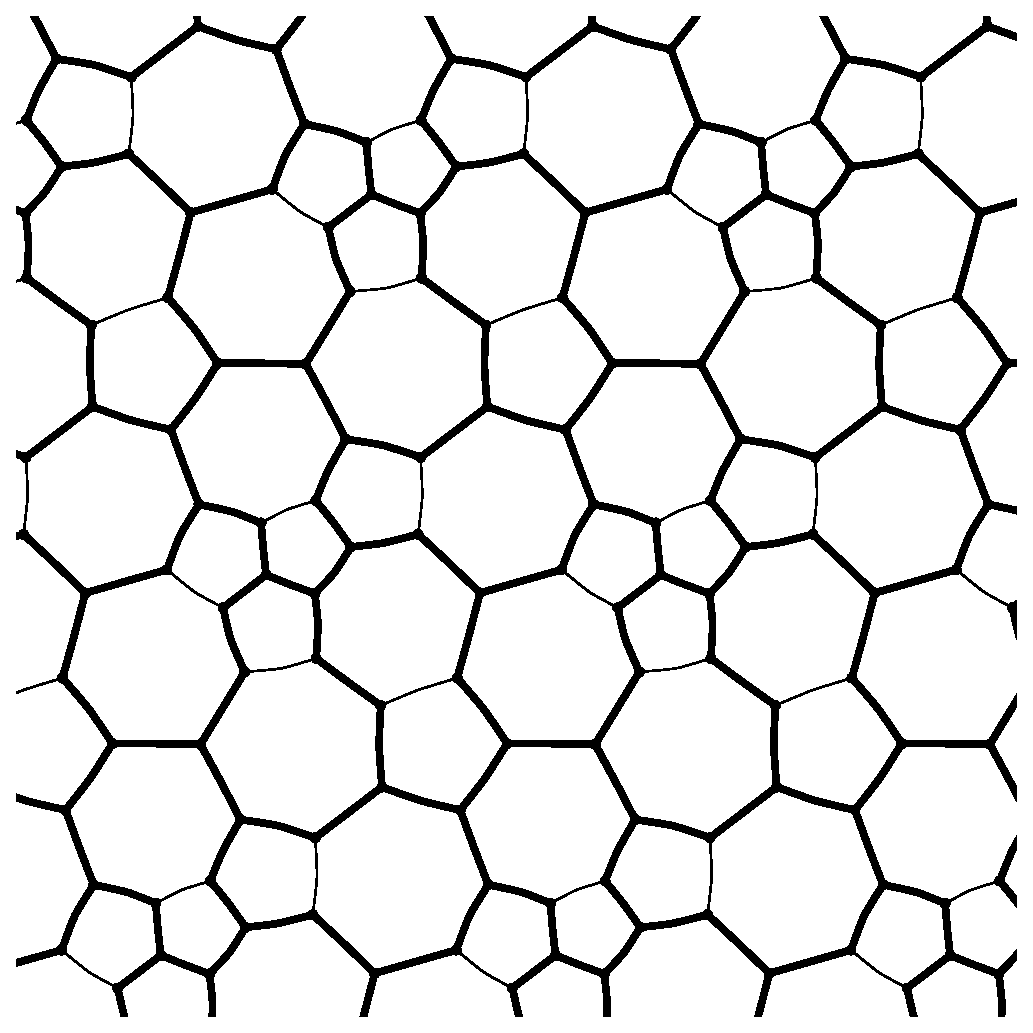
\epsfig{height=25mm, file=EPSdatabase/CASE_g1_k3_n20_-_5_5_-_7_5/PLOT_1_PL_1_cm_1_-_1_p1.eps}
%\par 
%20, $cm$ (p1)\\
%$\vec{p}$=$(5,5)$
%\end{minipage}
%\begin{minipage}[b]{2.4cm}\centering
%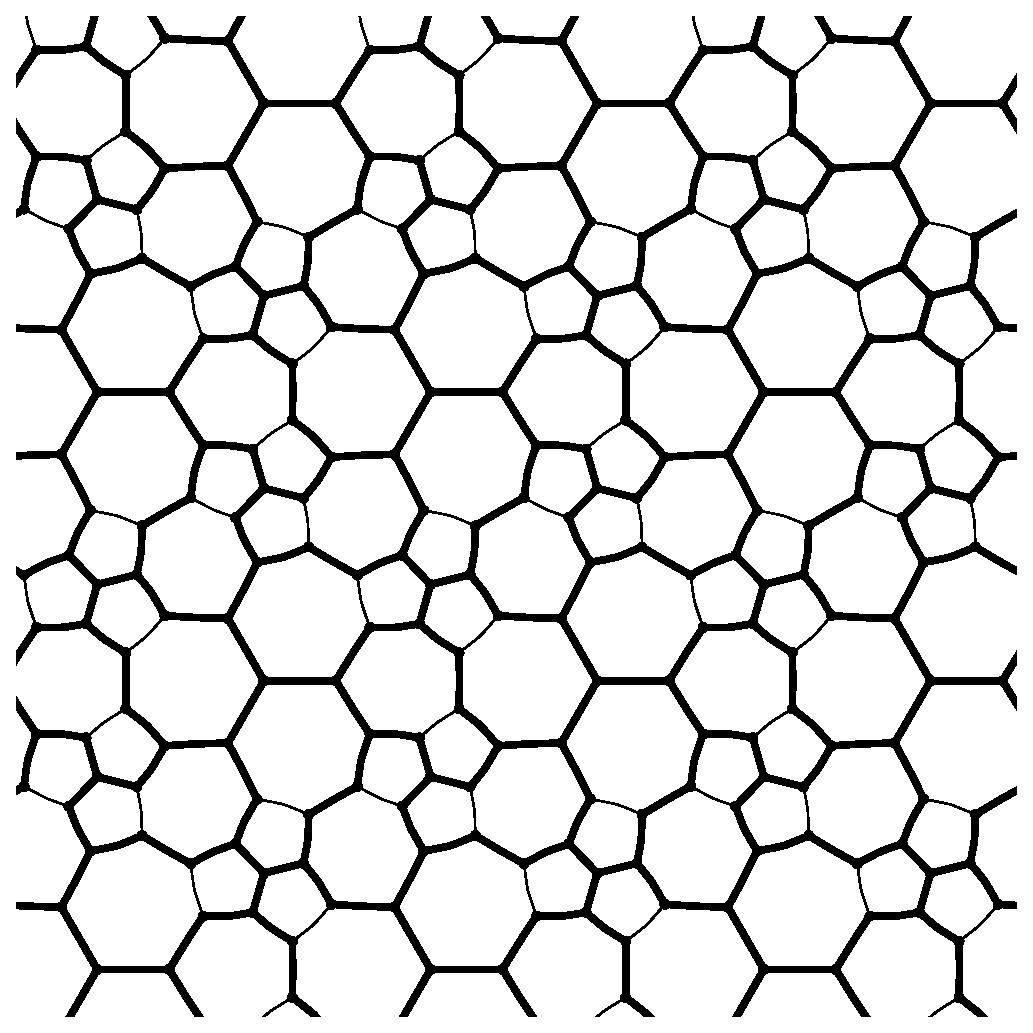
\epsfig{height=24mm, file=EPSdatabase/CASE_g1_k3_n24_-_5_6_-_7_6/PLOT_1_PL_22_p31m_1_-_3_p3.eps}
%\par 
%24, $p31m$ (p3)\\
%$\vec{p}$=$(6,6)$
%\end{minipage}
%\begin{minipage}[b]{2.4cm}\centering
%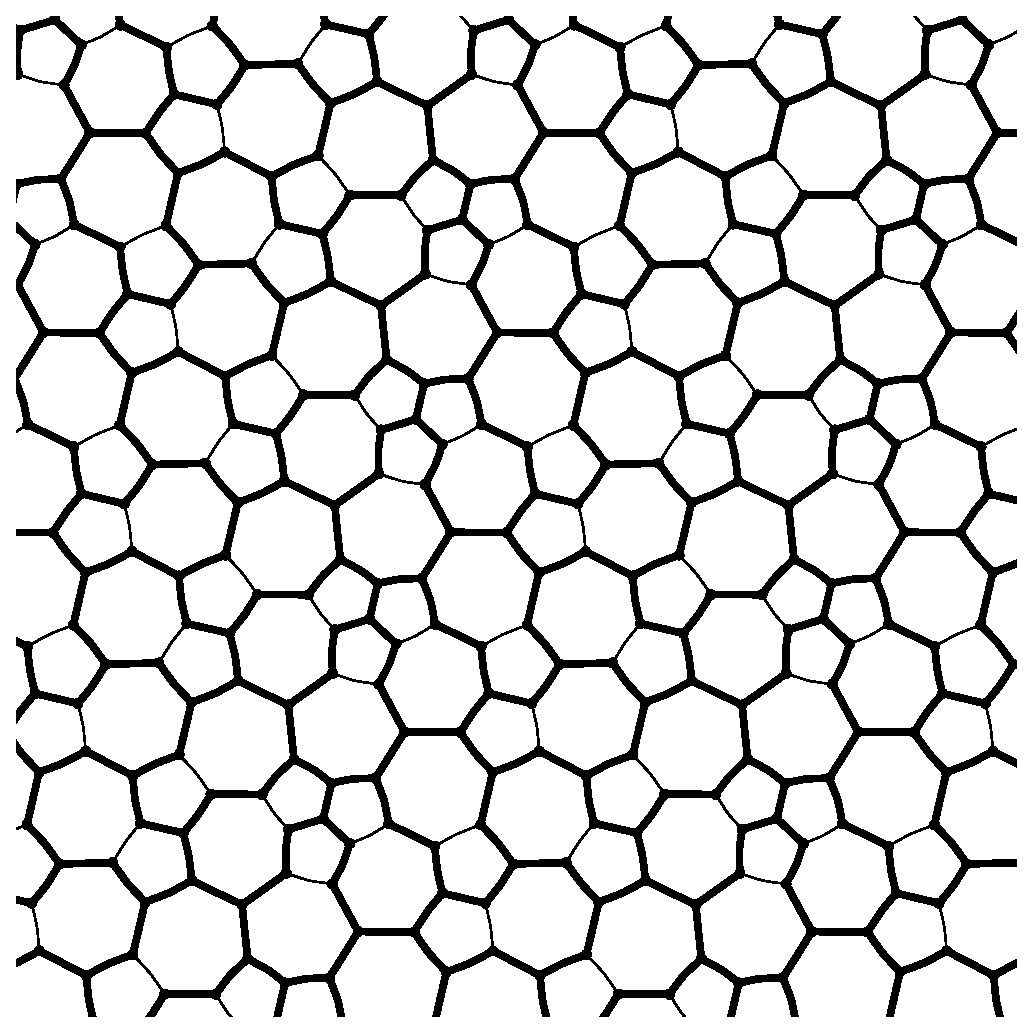
\epsfig{height=24mm, file=EPSdatabase/CASE_g1_k3_n28_-_5_7_-_7_7/PLOT_1_PL_4_cm_1_-_2_cm.eps}
%\par 
%28, $cm$ (cm)\\
%$\vec{p}$=$(7,7)$
%\end{minipage}
%\begin{minipage}[b]{2.7cm}\centering
%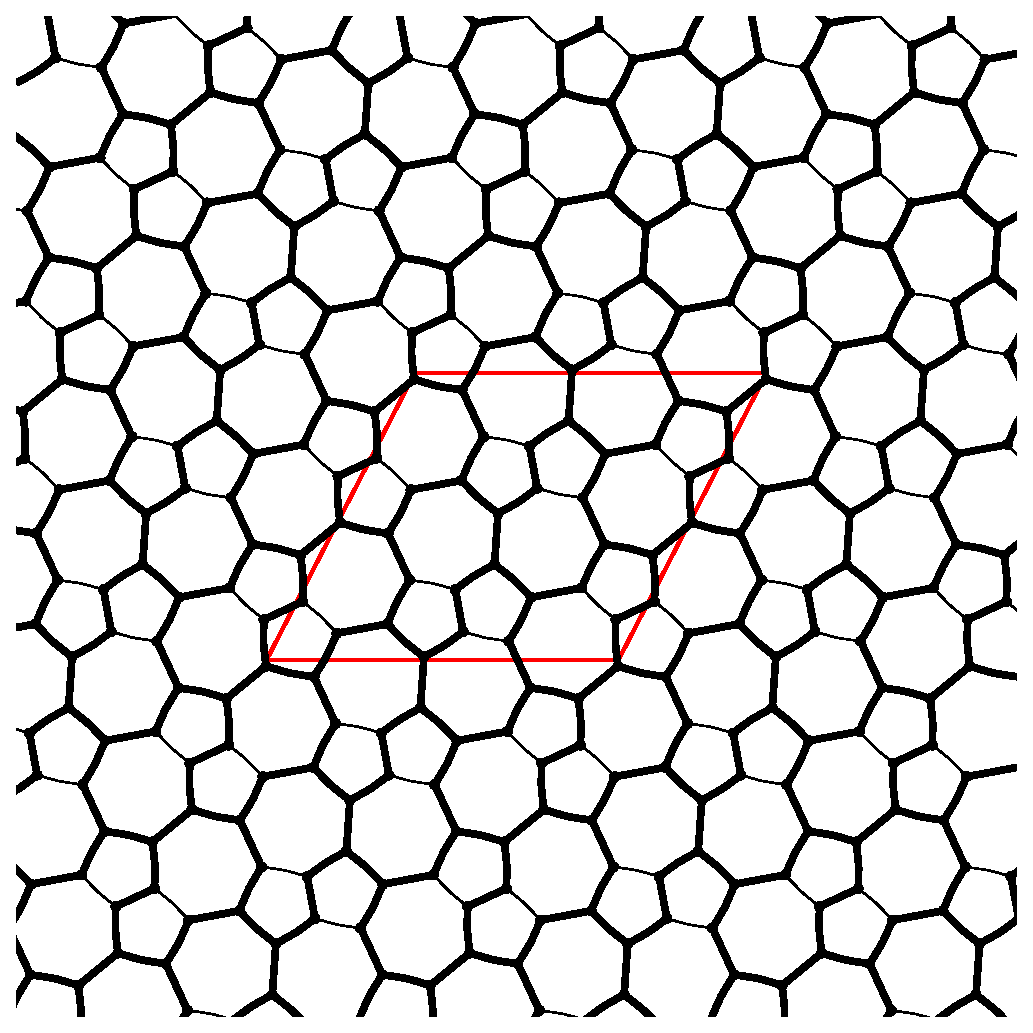
\epsfig{height=25mm, file=EPSdatabase/CASE_g1_k3_n32_-_5_8_-_7_8/PLOT_1_PL_4_p2gg_1_-_32_p2gg.eps}
%\par 32, $p2gg$ (p2gg)\\
%$\vec{p}$=$(8,8)$ \end{minipage}
%\begin{minipage}[b]{2.7cm}\centering
%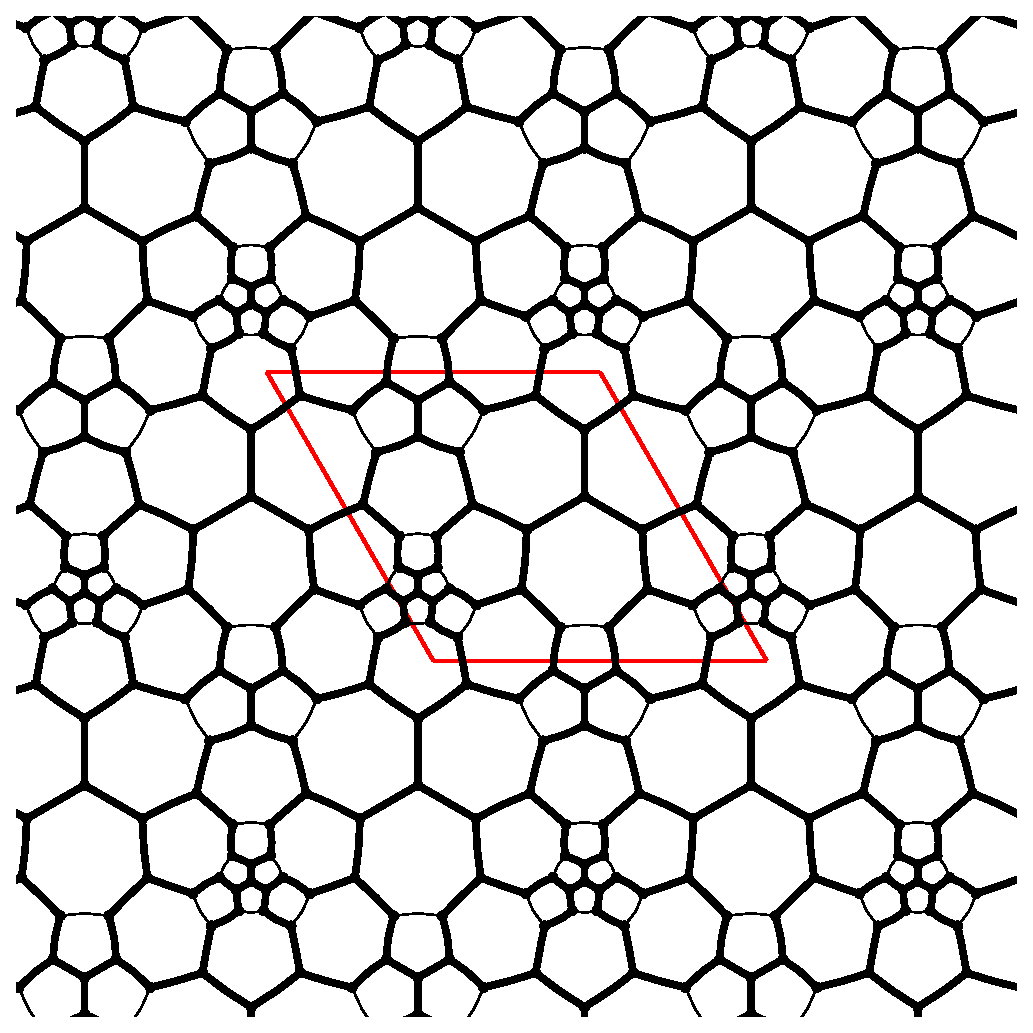
\epsfig{height=25mm, file=EPSdatabase/CASE_g1_k3_n36_-_5_9_-_7_9/PLOT_1_PL_3_p3m1_1_-_1_p3m1.eps}
%\par 36, $p3m1$ (p3m1)\\
%$\vec{p}$=$(9,9)$
%\end{minipage}
%\end{center}
%\end{frame}









\frame{
\begin{center}
{\Huge 
\begin{tabular*}{6cm}{c}
\\[-0.5cm]
\textcolor{blue}{I. }\textcolor{red}{Enumeration}\\
\textcolor{red}{methods}
\end{tabular*}
}
\end{center}
}




\frame{
  \frametitle{List of problems to be solved}

\begin{itemize}
\item Problem I is:
\begin{itemize}
\item We have a list of $p'_a$ $a$-gonal faces and $p'_b$ $b$-gonal faces
\item We want to find all possible lego pieces
\end{itemize}
This is done, when possible, by exhaustive enumeration by adding pieces one after the other in all configurations.
\item Problem II is:
\begin{itemize}
\item We have a list of maps on the sphere or on torus
\item We want to find all legos that occur here.
\end{itemize}
This kind of enumeration is limited to the $(\{a,b\},k)$-map classes for which enumeration is feasible and there is a program for it.

\item Problem III is:
\begin{itemize}
\item We have a set of lego pieces
\item We want to find all the ways in which they can fit together.
\end{itemize}
This kind of method is a priori more clever since we build first the list of pieces and then put them together.

\end{itemize}

}


\frame{
  \frametitle{List of feasible cases}

\begin{itemize}
\item The program {\tt CPF} (by Thomas Harmuth, Master Thesis) can enumerate the $(\{a,b\},3)$-spheres with a fixed number of vertices and $a\geq 3$, which are the most important cases.
\item The program {\tt CGF} (by Thomas Harmuth, PhD Thesis) can enumerate all the $(\{a,b\},3)$-maps of fixed genus and number of vertices with $a\geq 3$.
\item The program {\tt ENU} can enumerate the $(\{a,b\},4)$-spheres with fixed number of vertices and $a\geq 3$.
\item The program {\tt plantri} can do specific plane graph enumeration but it is much slower and hard to use.
\end{itemize}
In all other cases, we are on our own to get the maps. Possible methods is to reduce to one of the above classes.
For some cases, e.g. $(\{3,7\},3)$-spheres with $68$ vertices, the program cannot terminate. Reductions are then needed.
}





\frame{
  \frametitle{Exact covering problem}

Problem is:
\begin{itemize}
\item Given $n$ points and $m$ subsets $S_1$, \dots, $S_m$ of $\{1, \dots, n\}$
\item to find all partitions of $\{1, \dots, n\}$ by subsets $S_i$.
\end{itemize}
Features:
\begin{itemize}
\item The existence problem can be formulated as Integer Programming Problem and it is NP.
\item It is an exhaustive enumeration problem and so harder a priori.
\item Fortunately, there exist the program {\tt LibExact} by Kaski and Pottonen which implements a very fast enumeration procedure using ``dancing links''.
\item It does not uses symmetry so we have to do isomorphism checks afterwards.
\end{itemize}
}


\frame{
  \frametitle{Satisfiability problems SAT}
A satisfiability problem (SAT) is a problem of the type:
\begin{itemize}
\item A number $n$ of variables $v_1$, \dots, $v_n$ that can be true or false.
\item A number of \textcolor{red}{clauses} of the form
\begin{equation*}
w_1 \vee w_2 \vee \dots \vee w_p \mbox{~with~} w_j = v_{i_j} \mbox{~or~} \overline{v_{i_j}}.
\end{equation*}
\item A set of clauses to be satisfied, i.e.
\begin{equation*}
c_1 \wedge c_2 \wedge\dots \wedge c_M.
\end{equation*}
\end{itemize}
The goal is to find whether there exist a set of variables that satisfies all the clauses.

The program {\tt minisat} can check satisfiability very fast despite SAT being a NP problem.
This allows to solve some combinatorial problems. We can also enumerate all the solutions of a SAT problem.
}


\frame{
  \frametitle{SAT for legos}
SAT problems can be used to solve Sudoku, N-queens problems and generally all kinds of combinatorial problems. What about legos:
\begin{itemize}
\item We take a set of $N$ lego pieces, each identical and each having $p$ sides.
\item We need to put the condition of adjacency between the sides. So, this makes about $(Np)^2$ variables.
\item We have conditions around the edges since we want the degree to be a specified value of say $k$.
\item But we cannot handle questions of connectivity.
\end{itemize}
In general the approach failed and this seems to be generally the experience when using SAT to solve combinatorial problems such as $t$-designs, distance regular graphs, etc.
}


\frame{
  \frametitle{Direct enumeration method}

So, instead of SAT, we used a more classical enumeration method:
\begin{itemize}
\item The idea is to take one lego and add pieces one at a time until the obtained graph is complete.
\item In the case of place graph, one can prove that we can add the pieces so that at all time the space that is not covered is connected.
\item The method is typical backtrack enumeration and is all done in C++.
\end{itemize}
Results:
\begin{itemize}
\item The method generally works for up to say $8$-$12$ lego pieces.
\item This allows to solve many cases.
\end{itemize}

}








\frame{
\begin{center}
{\Huge 
\begin{tabular*}{6cm}{c}
\\[-0.5cm]
\textcolor{blue}{I. }\textcolor{red}{Graph}\\
\textcolor{red}{drawing}
\end{tabular*}
}
\end{center}
}


\frame{
  \frametitle{Problematic}

\begin{itemize}
\item The problem that we have is how to represent a graph on the plane or torus in a practical way.
\item The difficulty is how to represent $1$-gons and $2$-gons, which most method do not.
\item Another issue is that many methods require the graph to be $3$-connected, which is a strong requirement.
\end{itemize}
Additional wishes
\begin{itemize}
\item We want the program to be as fast as possible. Drawing should be a non-issue
\item We want details to be clearly visible.
\item We want the symmetries to be visible.
\end{itemize}
}

\begin{frame}[fragile]
  \frametitle{Representation of oriented maps}

\begin{itemize}
\item General maps are best represented via flag system (buildings, chamber system, etc.)
\item For oriented maps, we can use a simpler yet equivalent system: directed edge.
\item Directed edge are basically a pair $(v, e)$ with $v$ a vertex and $e$ an edge.
\item Given a directed edge $\overrightarrow{e}$ we can build the next directed edge $n(\overrightarrow{e})$ around the vertex (in trigonometric order) and the inverse directed edge $i(\overrightarrow{e})$
\item Vertices, edges and faces the correspond to the orbits of the permutations $n$, $i$ and $n\circ i$ on the set of directed edges.
\end{itemize}
Example:
\begin{verbatim}
16
 8 11 4 9 2 15 14 13 0 3 12 1 10 7 6 5
 1 2 3 0 5 6 7 4 9 10 11 8 13 14 15 12
\end{verbatim}

  
\end{frame}








\frame{
  \frametitle{Existing approaches}

\begin{itemize}
\item \textcolor{red}{Tutte}: He proposed to use eigenvectors of the adjacency matrix in order to provide embeddings. The method works well for plane graphs but suffer from one key problem: the inner faces tend to be very small and not visible. Only for plane graphs.
\item \textcolor{red}{Dress,Harmuth,Delgado Friedrichs,Brinkmann}: The {\tt CaGe} program uses an iterative process in order to get the embedding. A priori only for plane graphs.
\item \textcolor{red}{Mohar}: Primal-Dual circle packings provide a good theoretical based approach for finding the embeddings. It works for plane graph, torus and hyperbolic maps.
\item Force directed graphs. A physical functional such as
  \begin{equation*}
  F = \sum_{e=(i,j) \in E(G)} f(\Vert x_i - x_j\Vert)
  \end{equation*}
  and we minimize over the embedding.
\end{itemize}
}


\frame{
  \frametitle{Issues and features}

Features:
\begin{itemize}
\item All above techniques will respect symmetries since they are based on minimization procedure. But sometimes the number of iterations needs to be adjusted.
\item All coordinates are obtained by iteration procedures. We cannot do exact arithmetic computations.
\end{itemize}
  
Issues:
\begin{itemize}
\item Some technique requires $3$-connectivity of the graph
\item All fail to work for $2$-gons and $1$-gons.
\item Convergence might take a long time to achieve.
\item Some details of the graph might be very hard to see in the final drawing. According to the cases
\begin{itemize}
\item For the plane graph, one factor is the proximity to the exterior face, another is the level of refinement.
\item For the torus, it is flat so the only problem is the level of refinement.
\item For the hyperbolic plane, the problem will necessarily occur in all reasonable representations such as Poincar\'e plane or similar.
\end{itemize}
\end{itemize}

}







\frame{
  \frametitle{Primal-Dual circle packings}
The idea is to put circles in the vertex center and faces such that
\begin{itemize}
\item If any two vertices $v$ and $v'$ are adjacent then the corresponding circles are tangent.
\item For any face the circle is tangent to the edges.
\end{itemize}
\begin{center}
  \begin{minipage}[b]{4.5cm}
    \centering
    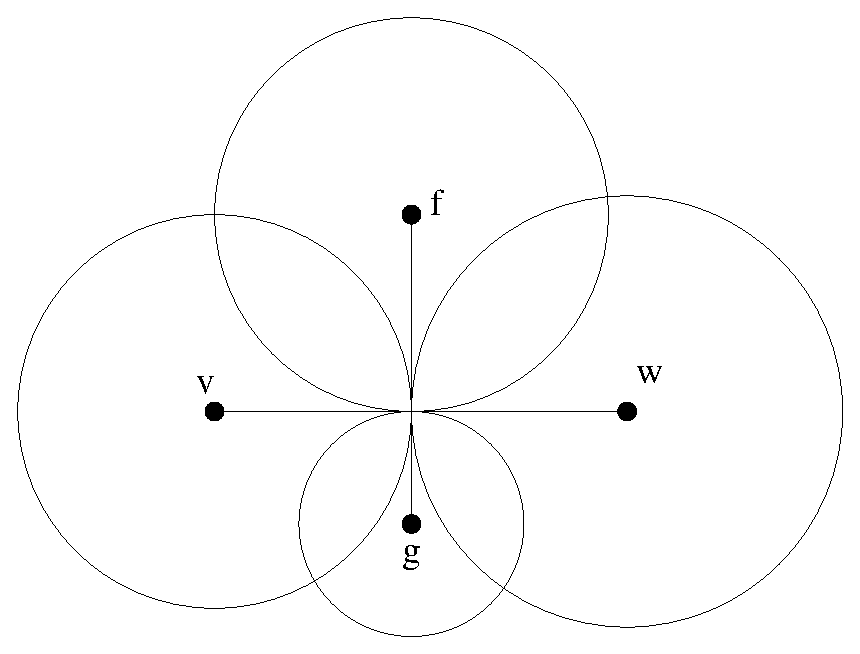
\epsfig{file=Intro/PrimalDualRepr.eps, width=5cm}\par
    The local picture of a primal-dual circle representation
  \end{minipage}
  \begin{minipage}[b]{4.5cm}
    \centering
    \resizebox{5cm}{!}{\rotatebox{0}{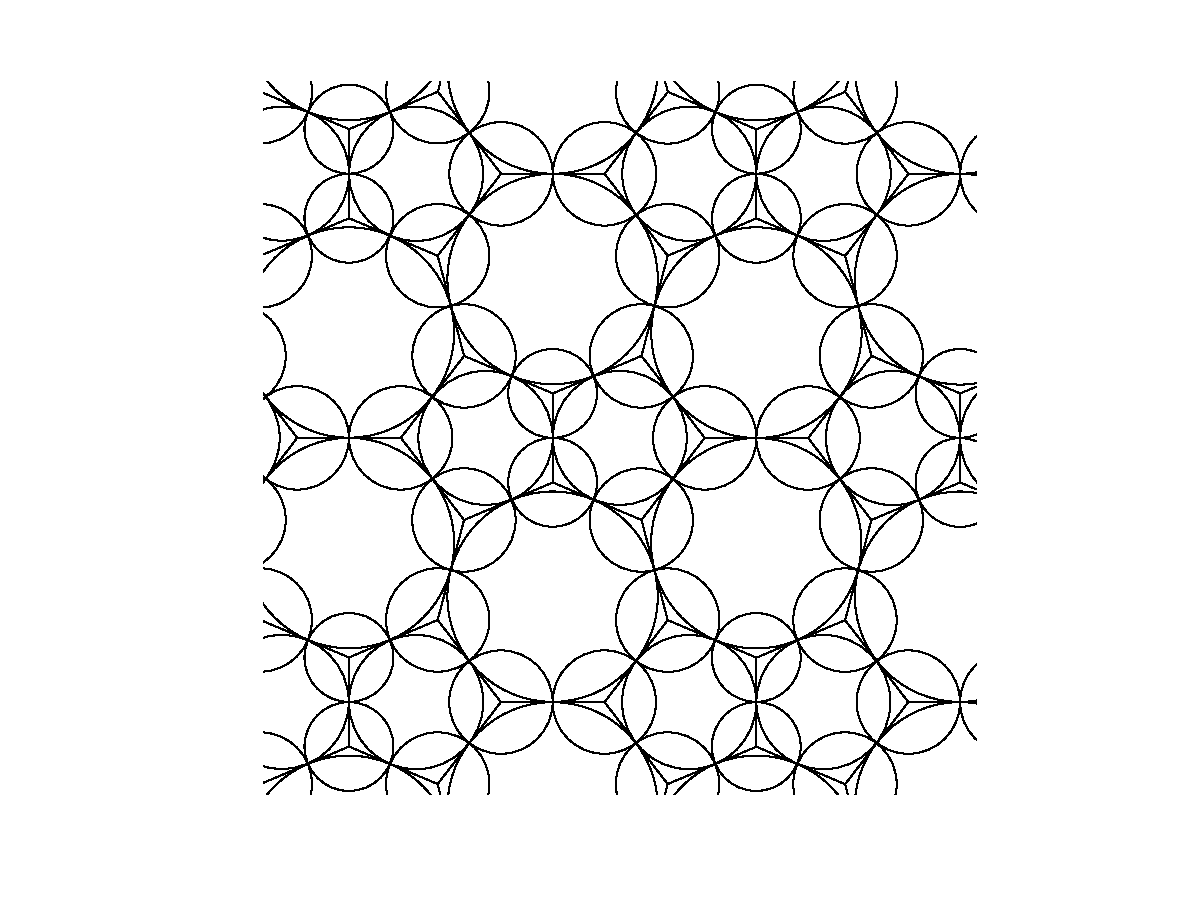
\includegraphics{Intro/CirclesEdges.eps}}}\par
    The edges, circle and face circles of a primal-dual representation
  \end{minipage}
\end{center}
}



\frame{
  \frametitle{Primal-Dual circle packings: Equations and Numerics}
\begin{itemize}
\item In the case of torus, the equations that are satisfied are
  \begin{equation*}
  \pi = \phi_v = \sum_{uv \in E(Med^*(G))} \arctan\left(\frac{r_u}{r_v}\right)
  \end{equation*}
  for each vertex $v$ of the dual medial graph of $G$.
\item Bojan Mohar has given an algorithm for computing primal dual circle packings. It consists of computing
the defect at every node and increasing/decreasing the radius value according to $\phi_v > \pi$ or $\phi_v < \pi$. It is a geometric method but in some cases it is very slow.
\item Instead our approach is to use a variant of Newton method: We choose the direction of change
  from the Newton iteration solver and we adjust the amount of change so that we remain in the allowed
  region of circles of positive radius.
  \begin{equation*}
  x^{(n+1)} = x^{(n)} - c \frac{f(x^{(n)})}{f'(x^{(n)})} \mbox{~with~} 0<c \leq 1
  \end{equation*}
  
\end{itemize}
}



\frame{
  \frametitle{Refinement techniques}

\begin{itemize}
\item The primal-dual technique requires $3$-connectivity and will not work with $2$-gons and $1$-gons.
\item The technique is to refine it. First for a map $M$ we replace it with the order complex map $Ord(M) = Trunc(Med(M))$.
\item Then we insert a vertex and each edge.
\item Finally, we put a vertex on each face and connect it with all incident vertices.
\item The resulting triangulation is $3$-connected.
\end{itemize}

\begin{center}
\hspace{-2cm}
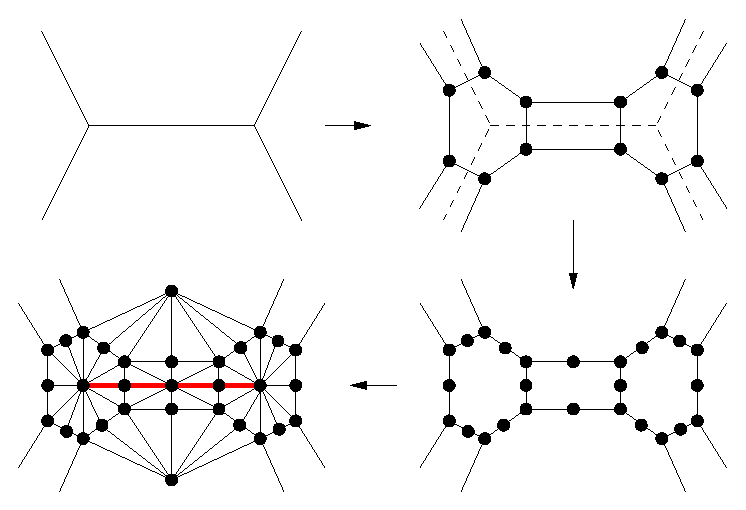
\epsfig{file=DecompositionGraphs/FullScheme.eps, width=6.0cm}\par
\end{center}
  
}




\frame{
  \frametitle{Symmetric representation}

\begin{itemize}
\item For plane graph, we want to represent the maps with the maximum amount of symmetry.
\item In practical matter if we have an axis of symmetry of order $N$ then we want it visible.
\item If the axis pass by a vertex or an edge then we put it to infinity.
\end{itemize}
Examples:
\begin{center}
\begin{minipage}[b]{3.5cm}
\centering
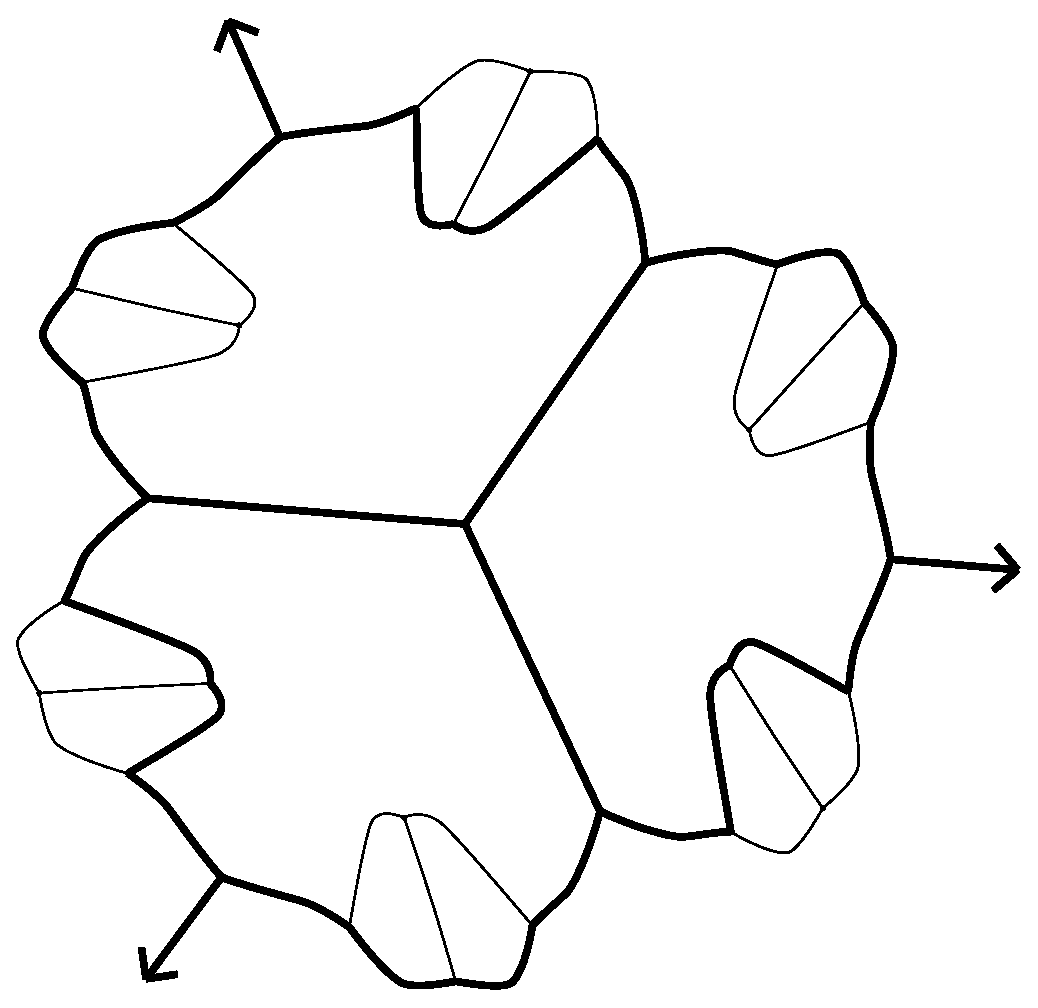
\epsfig{file=ExternalFaces/PLOT_1_PL_2_D3d_1_-_1_S6.eps, width=3.5cm}\par
On vertex
\end{minipage}
\begin{minipage}[b]{3.5cm}
\centering
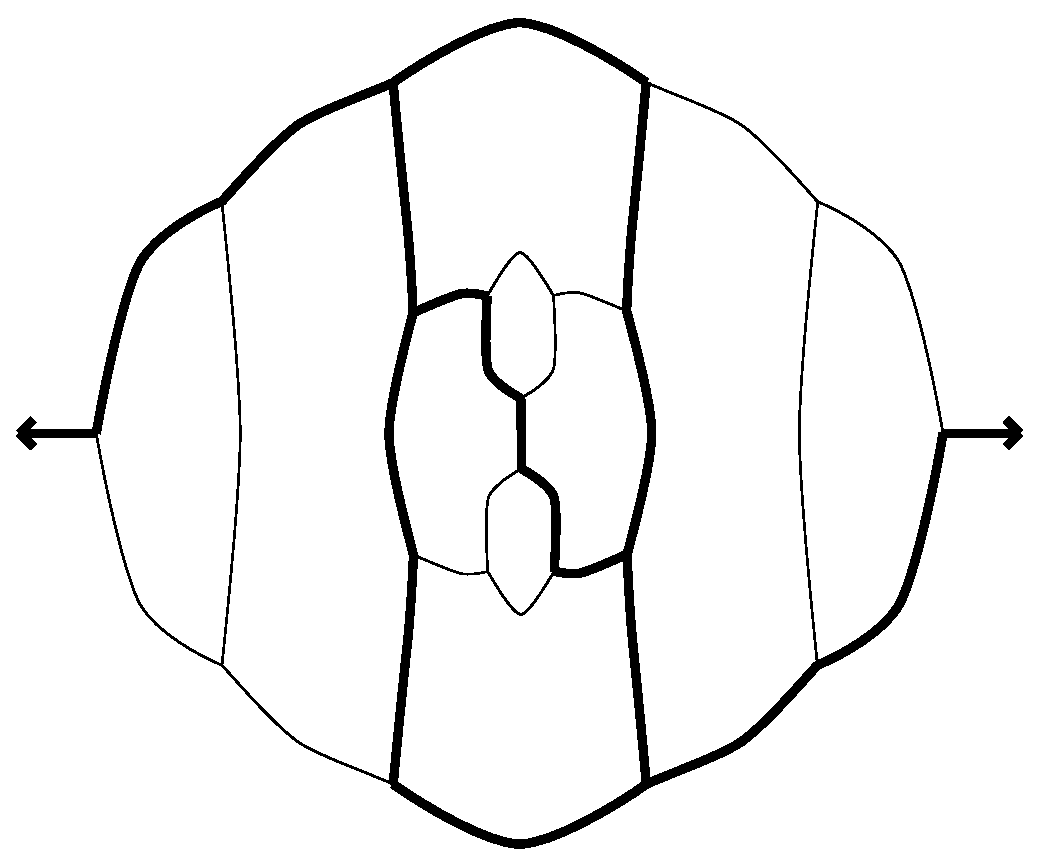
\epsfig{file=EPSdatabase/CASE_g0_k3_n20_-_3_4_-_6_8/PLOT_1_PL_2_D2d_1_-_1_D2.eps, width=3.5cm}\par
On edge
\end{minipage}
\begin{minipage}[b]{3.5cm}
\centering
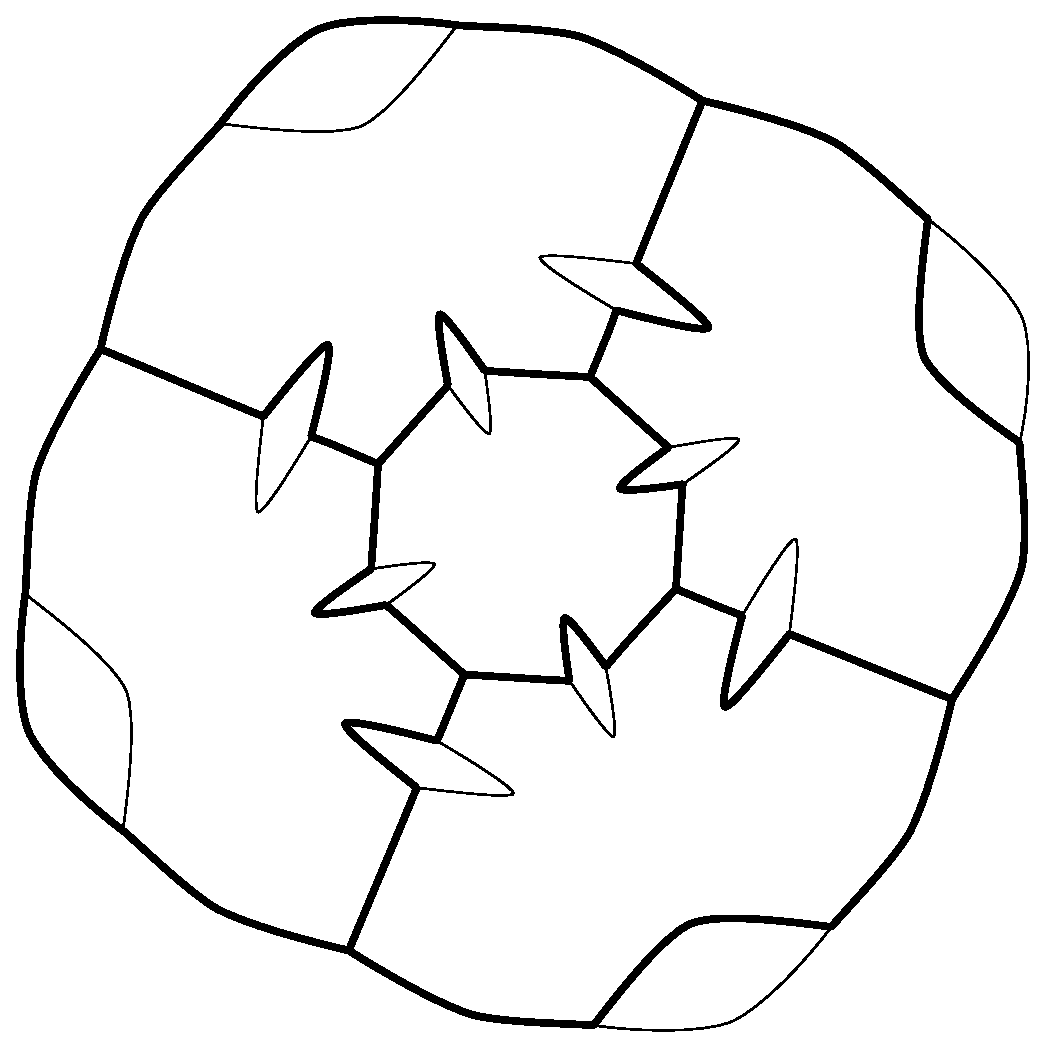
\epsfig{file=ExternalFaces/PLOT_2_PL_6_Oh_2_-_1_S6.eps, width=3.5cm}\par
On face
\end{minipage}
\end{center}
}



\frame{
  \frametitle{CaGe process}

  \begin{itemize}
  \item Suppose that we have a point $x$ and $m$ adjacent points $x^1$, \dots, $x^m$ then for the CaGe process we have the equation
    \begin{equation*}
    x = \frac{1}{\sum_{i=1}^m A^2_T(x,x^i, x^{i+1})} \sum_{i=1}^m A^2_T(x, x^i, x^{i+1}) \frac{x + x^i + x^{i+1}}{3}
    \end{equation*}
with $A_T(x, y, z)$ the area of the triangle of vertices $x$, $y$ and $z$.
\item The equation is solved by fixed point iterations.
%\item For the plane graph, we simply put the vertices of the exterior face in a circle.
\item Plane graph: put the vertices of the exterior face in a circle.
\item Torus map: first guess obtained by primal dual circle packing and then apply the CaGe process.
\end{itemize}

\begin{center}
\begin{minipage}[b]{4.5cm}
\centering
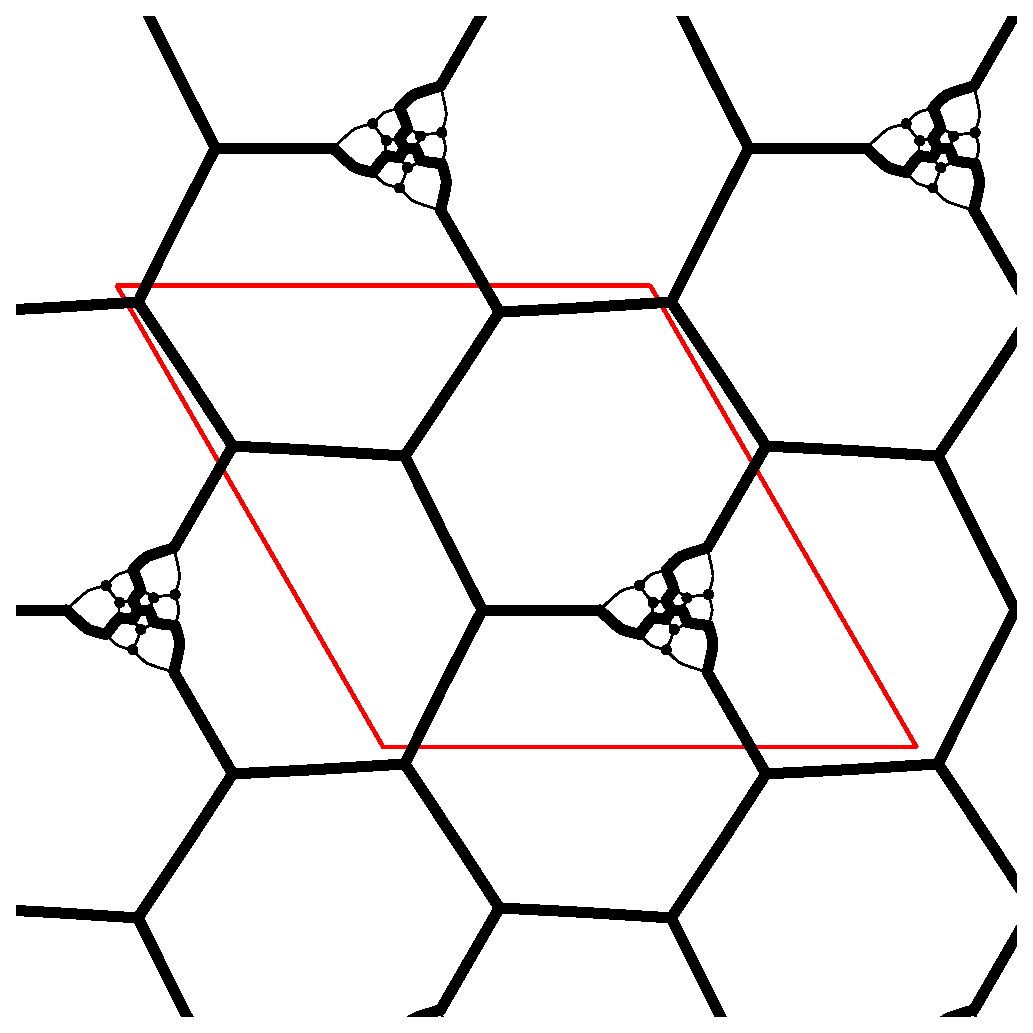
\epsfig{file=Examples/PLOT_1_PL_1_p31m_1_-_1_p3_PD.eps, width=3.5cm}\par
Primal dual
\end{minipage}
\begin{minipage}[b]{4.5cm}
\centering
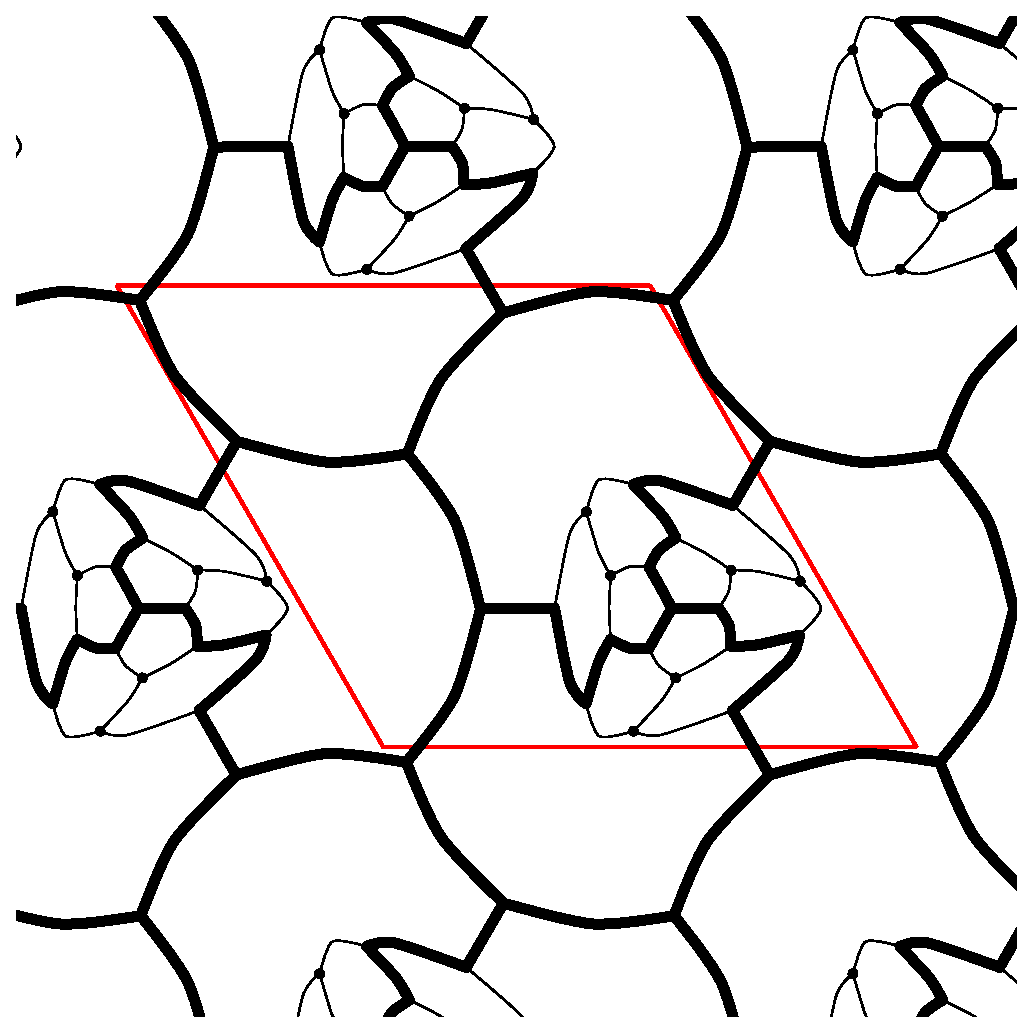
\epsfig{file=Examples/PLOT_1_PL_1_p31m_1_-_1_p3_CAGE.eps, width=3.5cm}\par
CaGe process
\end{minipage}
\end{center}
}















\frame{
  \frametitle{Problem of $1$-gons}

\begin{itemize}
\item Our approach of auxiliary graphs works fairly well with $2$-gons.
\item But with $1$-gons, we tend to get far smaller faces than expected.
\item The empirical solution is to rescale the $1$-gons by large factors (say $200$) so that they become visible.
\end{itemize}
\begin{center}
\begin{minipage}{4.5cm}\centering
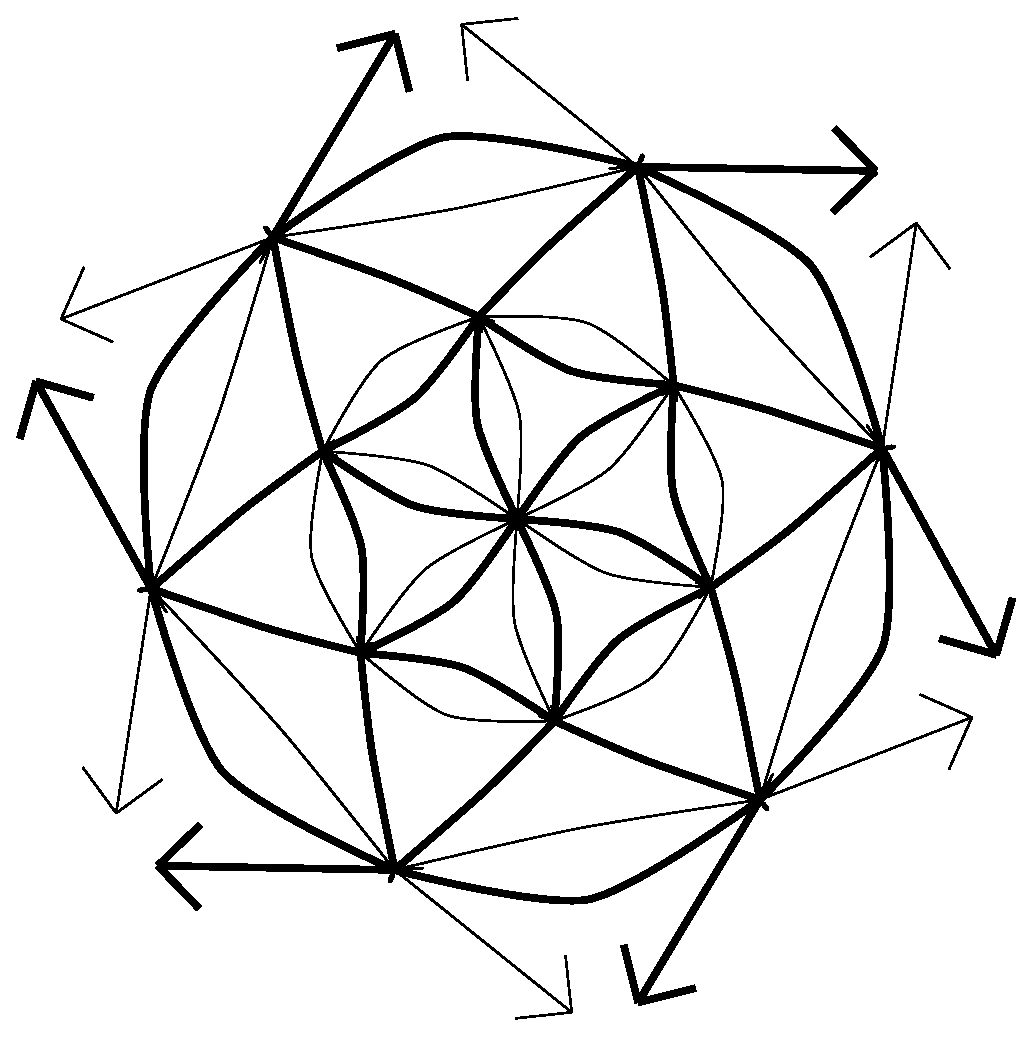
\epsfig{height=4.5cm, file=Examples/PLOT_1_PL_1_D6_1_-_1_D6_normal.eps}\par
normal
\end{minipage}
\begin{minipage}{4.5cm}\centering
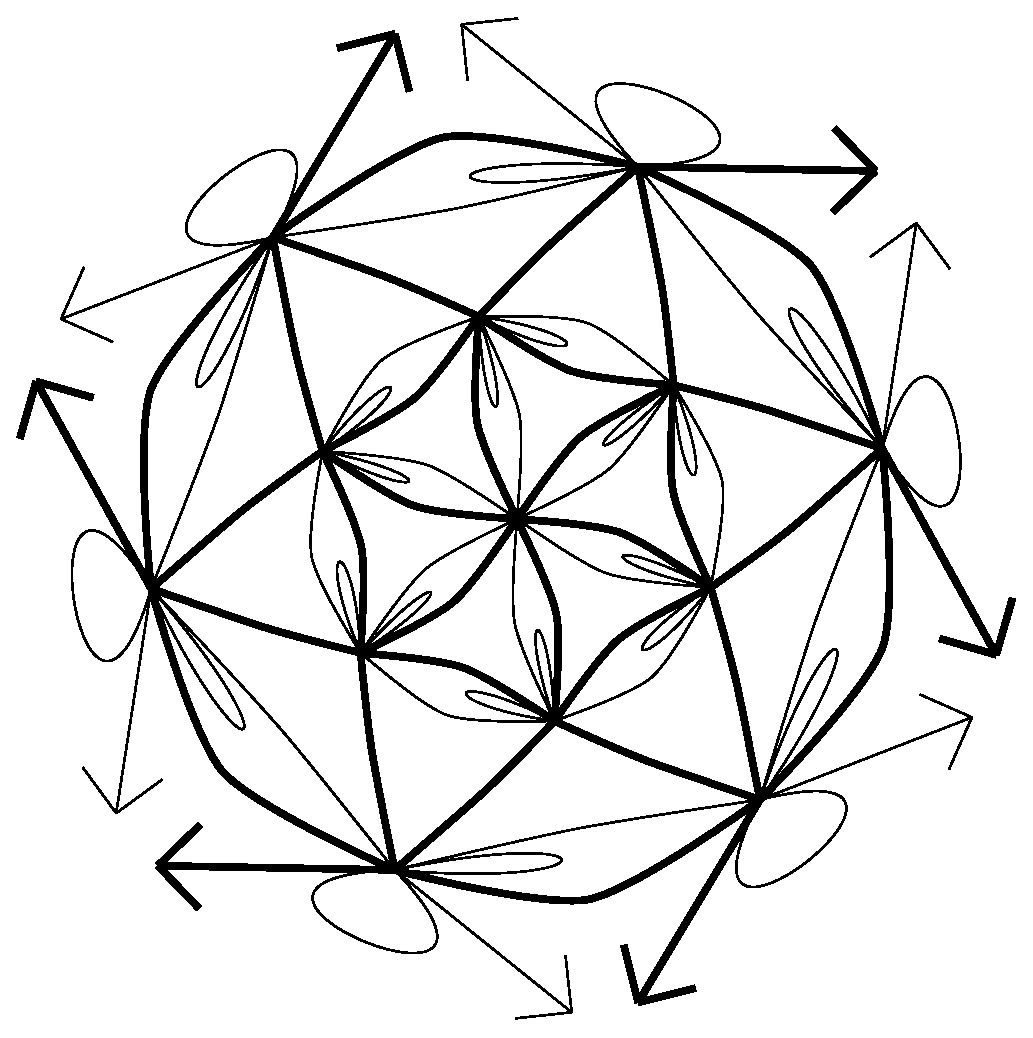
\epsfig{height=4.5cm, file=Examples/PLOT_1_PL_1_D6_1_-_1_D6_expand.eps}\par
expanded
\end{minipage}

\end{center}

}



\frame{
  \frametitle{Software availability}

\begin{itemize}
\item Source code is available at
  \begin{center}
  https://github.com/MathieuDutSik/Plot\_orientedmap
  \end{center}
\item Code written in {\tt C++11} language.
\item Uses the Eigen library for matrix computations.
\item Input file in Namelist, fortran style input.
\item Output file in {\tt svg} (Scalable Vector Graphics) to be used on web page or in Inkscape.
\end{itemize}
}








\end{document}
